% presentation
\documentclass{beamer}
\usetheme[height=7mm]{Rochester}
\usecolortheme{rose}

% handout

%\documentclass[handout]{beamer}
%\usepackage{pgfpages} \pgfpagesuselayout{8 on 1}[a4paper]

%\documentclass[mathserif]{article}
%\usepackage{beamerarticle}

\usepackage{amsmath}
\usepackage{comment}
\usepackage{amssymb,amsfonts}
\usepackage[T1]{fontenc}
\usepackage{lmodern}
\usepackage{tikz}
\usepackage{simpsons}
\usepackage{marvosym}
\usepackage{color}
\usepackage{multirow}
\usepackage{pgffor}
\usepackage[slide,algoruled,titlenumbered,vlined,noend,linesnumbered,]{algorithm2e}

\usefonttheme{structurebold}

\setbeamertemplate{footline}[frame number]
\setbeamertemplate{navigation symbols}{}
\setbeamerfont{smallverb}{size*={73}}
\usefonttheme[onlymath]{serif}
\setbeamertemplate{theorems}[numbered]
\newtheorem{construction}[theorem]{Construction}
\newtheorem{proposition}[theorem]{Proposition}

\AtBeginSection[] { 
  \begin{frame} 
    \frametitle{Content} 
    \tableofcontents[currentsection]
  \end{frame} 
  \addtocounter{framenumber}{-1} 
}

\usetikzlibrary[shapes.arrows]
\usetikzlibrary{shapes.geometric}
\usetikzlibrary{backgrounds}
\usetikzlibrary{positioning}
\usetikzlibrary{calc}
\usetikzlibrary{intersections}
\usetikzlibrary{fadings}
\usetikzlibrary{decorations.footprints}
\usetikzlibrary{patterns}
\usetikzlibrary{shapes.callouts}
\usetikzlibrary{fit}
%handout

\providecommand{\abs}[1]{\lvert#1\rvert}

\tikzset{every picture/.style={line width=1pt,show background rectangle},background rectangle/.style={fill=blue!10,rounded corners=2ex}}

\author{Yu Zhang}
\institute{Harbin Institute of Technology}
\date[Crypt'16A]{Cryptography, Autumn, 2016}

%% presentation
\documentclass{beamer}
\usetheme[height=7mm]{Rochester}
\usecolortheme{rose}

% handout

%\documentclass[handout]{beamer}
%\usepackage{pgfpages} \pgfpagesuselayout{8 on 1}[a4paper]

%\documentclass[mathserif]{article}
%\usepackage{beamerarticle}

\usepackage{amsmath}
\usepackage{comment}
\usepackage{amssymb,amsfonts}
\usepackage[T1]{fontenc}
\usepackage{lmodern}
\usepackage{tikz}
\usepackage{simpsons}
\usepackage{marvosym}
\usepackage{color}
\usepackage{multirow}
\usepackage{pgffor}
\usepackage[slide,algoruled,titlenumbered,vlined,noend,linesnumbered,]{algorithm2e}

\usefonttheme{structurebold}

\setbeamertemplate{footline}[frame number]
\setbeamertemplate{navigation symbols}{}
\setbeamerfont{smallverb}{size*={73}}
\usefonttheme[onlymath]{serif}
\setbeamertemplate{theorems}[numbered]
\newtheorem{construction}[theorem]{Construction}
\newtheorem{proposition}[theorem]{Proposition}

\AtBeginSection[] { 
  \begin{frame} 
    \frametitle{Content} 
    \tableofcontents[currentsection]
  \end{frame} 
  \addtocounter{framenumber}{-1} 
}

\usetikzlibrary[shapes.arrows]
\usetikzlibrary{shapes.geometric}
\usetikzlibrary{backgrounds}
\usetikzlibrary{positioning}
\usetikzlibrary{calc}
\usetikzlibrary{intersections}
\usetikzlibrary{fadings}
\usetikzlibrary{decorations.footprints}
\usetikzlibrary{patterns}
\usetikzlibrary{shapes.callouts}
\usetikzlibrary{fit}
%handout

\providecommand{\abs}[1]{\lvert#1\rvert}

\tikzset{every picture/.style={line width=1pt,show background rectangle},background rectangle/.style={fill=blue!10,rounded corners=2ex}}

\author{Yu Zhang}
\institute{Harbin Institute of Technology}
\date[Crypt'16A]{Cryptography, Autumn, 2016}

%\input{1introduction.tex}
%\input{2perfectlysecret.tex}
%\input{3privatekey.tex}


\title{Introduction}

\begin{document}
\maketitle
\begin{frame}
\frametitle{Outline}
\tableofcontents
\end{frame}
\section{Cryptography and Modern Cryptography}
\begin{frame}\frametitle{What is Cryptography?}
\begin{itemize}
\item \textbf{Cryptography}: from Greek \emph{krypt\'os}, ``hidden, secret''; and \emph{gr\'{a}phin}, ``writing''.
\item \textbf{Cryptography}: the art of writing or solving codes.\\ (Concise oxford dictionary 2006)
\item \textbf{Codes}: a system of prearranged signals, especially used to ensure secrecy in transmitting messages. \\ (\emph{code word} in cryptography)
\item \textbf{1980s}: from Classic to Modern; from Military to Everyone.
\item \textbf{Modern cryptography}: the scientific study of techniques for securing digital information, transactions, and distributed computations.
\end{itemize}
\end{frame}
\section{The Setting of Private-Key Encryption}
\begin{frame}\frametitle{Private-Key Encryption}
\begin{itemize}
\item \textbf{Goal}: to construct a \textbf{ciphers} (encryption schemes) for providing secret communication between two parties sharing \textbf{private-key} (the symmetric-key) in advance.
\item \textbf{Implicit assumption}: there is some way of initially sharing a key in a secret manner.
\item \textbf{Disk encryption}: the same user at different points in time.
\end{itemize}
\end{frame}
\begin{frame}\frametitle{The Syntax of Encryption}
\begin{figure}
\begin{center}
\begin{tikzpicture}
\node (sender) {\Lisa};
\node (bart) [below of = sender] {Alice};
\node (enc) [draw, right of = sender, rounded corners=1ex,node distance = 2cm] {$\mathsf{Enc}$};
\node (k1) [above of = enc, node distance = 1cm] {$k$};
\node (c) [right of = enc, node distance = 2cm] {$c$};
\node (gen) [draw, above of = c, rounded corners=1ex,node distance = 1cm] {$\mathsf{Gen}$};
\node (adv) [below of = c, node distance = 1cm] {\Burns};
\node (burns) [below of = adv] {Adversary};
\node (dec) [draw, right of = c, rounded corners=1ex,node distance = 2cm] {$\mathsf{Dec}$};
\node (k2) [above of = dec, node distance = 1cm] {$k$};
\node (receiver) [right of = dec, node distance = 2cm] {\Left\Bart};
\node (lisa) [below of = receiver] {Bob};
\draw[-latex] (sender) -- (enc) node [midway, above] {$m$};
\draw (enc) -- (c); \draw[-latex] (c) -- (dec);
\draw[-latex] (dec) -- (receiver) node [midway, above] {$m$};
\draw[-latex] (k1) -- (enc);
\draw[-latex] (gen) -- (k1);
\draw[-latex] (gen) -- (k2);								
\draw[-latex] (k2) -- (dec);		
\end{tikzpicture}
\end{center}
\end{figure}
\begin{itemize}
\item key $k \in \mathcal{K}$, plaintext (or message) $m \in \mathcal{M}$, ciphertext $c \in \mathcal{C}$.
\item \textbf{Key-generation} algorithm~$k \gets \mathsf{Gen}$.
\item \textbf{Encryption} algorithm~$c:= \mathsf{Enc}_k(m)$.
\item \textbf{Decryption} algorithm~$m:= \mathsf{Dec}_k(c)$.
\item \textbf{Encryption scheme}: $\Pi = (\mathsf{Gen}, \mathsf{Enc}, \mathsf{Dec})$.
\item \textbf{Basic correctness requirement}: $\mathsf{Dec}_k(\mathsf{Enc}_k(m)) = m$.
\end{itemize}
\end{frame}
\begin{frame}\frametitle{Securing Key vs Obscuring Algorithm}
\begin{itemize}
\item Easier to maintain secrecy of a short key.
\item In case the key is exposed, easier for the honest parties to change the key.
\item In case many pairs of people, easier to use the same algorithm, but different keys.
\end{itemize}
\begin{alertblock}{Kerckhoffs's principle}
\begin{quote}
The cipher method must not be required to be secret, and it must be able to fall into the hands of the enemy without inconvenience.
\end{quote}	
\end{alertblock}
\end{frame}
\begin{frame}\frametitle{Why ``Open Cryptographic Design''}
\begin{itemize}
\item Published designs undergo public scrutiny are to be stronger.
\item Better for security flaws to be revealed by ``ethical hackers''.
\item Reverse engineering of the code (or leakage by industrial espionage) poses a serious threat to security.
\item Enable the establishment of standards.
\end{itemize}
\end{frame}
\begin{frame}\frametitle{Attack Scenarios}	
\begin{itemize}
\item \textbf{Ciphertext-only}: the adversary just observes ciphertext
\item \textbf{Known-plaintext}: the adversary learns pairs of plaintexts/ciphertexts under the same key
\item \textbf{Chosen-plaintext}: the adversary has the ability to obtain the encryption of plaintexts of its choice
\item \textbf{Chosen-ciphertext}: the adversary has the ability to obtain the decryption of \textbf{other} ciphertexts of its choice
\item \textbf{Passive attack}: COA KPA
\begin{itemize}
\item because not all ciphertext are confidential
\end{itemize}
\item \textbf{Active attack}: CPA CCA
\begin{itemize}
\item when to encrypt/decrypt whatever an adversary wishes?
\end{itemize}
\end{itemize}	
\end{frame}
\section{Historical Ciphers and Their Cryptanalysis}
\begin{comment}
	\begin{frame}\frametitle{Why We Learn Broken Ciphers?}
	\begin{itemize}
	\item To understand the weaknesses of an ``ad-hoc'' approach
	\item To learn that ``simple'' approaches are unlikely to succeed
	\item To feel that ``we are smart enough to do some crypt-analyzing''
	\end{itemize}
	\end{frame}
\end{comment}

\begin{frame}[fragile]\frametitle{Caesar's Cipher}
\begin{quote}
If he had anything confidential to say, he wrote it in cipher, that is, by so changing the order of the letters of the alphabet, that not a word could be made out. If anyone wishes to \alert{decipher} these, and get at their meaning, he must \alert{substitute the fourth letter of the alphabet, namely D, for A}, and so with the others

\rightline{--Suetonius,``Life of Julius Caesar''}
\end{quote}
\begin{itemize}
	\item $\mathsf{Enc}(m)=m+3\mod 26$ \footnote{In fact the quote indicates that decryption involved rotating letters of the alphabet forward 3 positions, $\mathsf{Dec}(c)=c+3\mod 26$}
	\item \textbf{Weakness}: \alert{What is the key?}
\end{itemize}
\begin{exampleblock}{Example}
\verb|begintheattacknow|
%\verb|EHJLQWKHDWWDFNQRZ|
\end{exampleblock}
\end{frame}
\begin{frame}[fragile]\frametitle{Shift Cipher}
\begin{itemize}
\item $\mathsf{Enc}_k(m)=m+k\mod 26$
\item $\mathsf{Dec}_k(c)=c-k\mod 26$
\item \textbf{Weakness}: Fragile under \textbf{Brute-force attack} (exhaustive search)
\end{itemize}
\begin{exampleblock}{Example: Decipher the string}	
\verb|EHJLQWKHDWWDFNQRZ|
\end{exampleblock}
\begin{alertblock}{Sufficient Key Space Principle}
Any secure encryption scheme must have a key space that is not vulnerable to exhaustive search.\footnote{If the plaintext space is larger than the key space.}
\end{alertblock}
\end{frame}
\begin{frame}\frametitle{Index of Coincidence (IC) Method (to find $k$)}
\textbf{Index of Coincidence (IC)}: the probability that two randomly selected letters (pick-then-return) will be identical.

Let $p_i$ denote the probability of $i$th letter in English text.
\[I \overset{\text{def}}{=}\sum_{i=0}^{25} p_i^2 \]
\begin{exampleblock}{Example}
What's the IC of `apple'?
\end{exampleblock}

For a long English text, the IC is $\approx 0.065$.
For $j = 0, 1, \dotsc , 25$, $q_j$ is the probability of $j$th letter in the ciphertext.
\[I_j \overset{\text{def}}{=}\sum_{i=0}^{25} p_i \cdot q_{i+j}\]
\alert{Q: For shift cipher, if $j = k$, then $I_j \approx$ ?}

\end{frame}
\begin{frame}[fragile]\frametitle{Mono-Alphabetic Substitution}
\begin{itemize}
\item \textbf{Idea}: To map each character to a different one in an arbitrary manner.
\item \textbf{Strength}: Key space is large $\approx 2^{88}$. \alert{Q: how to count?}
\item \textbf{Weakness}: The mapping of each letter is fixed.
\end{itemize}
\begin{exampleblock}{Example}
\verb|abcdefghijklmnopqrstuvwxyz|\\
\verb|XEUADNBKVMROCQFSYHWGLZIJPT|

Plaintext: \verb|tellhimaboutme|\\
Ciphertext: \verb|??????????????|
\end{exampleblock}
\end{frame}
\begin{frame}[fragile]\frametitle{Attack with Statistical Patterns}
\begin{enumerate}
\item Tabulate the frequency of letters in the ciphertext.
\item Compare it to those in English text.
\item Guess the most frequent letter corresponds to \verb|e|, and so on.
\item Choose the plaintext that does ``make sense''. (Not trivial)
\end{enumerate}
\begin{table}
\begin{center}
\caption{Average letter frequencies for English-language text}
\begin{tabular}{|cc|cc|cc|cc|cc|} \hline
e & 12.7\% & t & 9.1\% & a & 8.2\% & o & 7.5\% & i & 7.0\%\\
n & 6.7\% & \_ & 6.4\% & s & 6.3\% & h & 6.1\% & r & 6.0\%\\
d & 4.3\% & l & 4.0\% & c & 2.8\% & u & 2.8\% & m & 2.4\%\\
w & 2.4\% & f & 2.2\% & g & 2.0\% & y & 2.0\% & p & 1.9\%\\
b & 1.5\% & v & 1.0\% & k & 0.8\% & j & 0.2\% & x & 0.2\%\\
q & 0.1\% & z & 0.1\% & & & & & &\\ \hline
\end{tabular}
\end{center}
\end{table}
\end{frame}
\begin{frame}[fragile]\frametitle{Example of Frequency Analysis (Ciphertext)}
\begin{verbatim}
LIVITCSWPIYVEWHEVSRIQMXLEYVEOIEWHRXEXIPFEMVEWHKVS
TYLXZIXLIKIIXPIJVSZEYPERRGERIMWQLMGLMXQERIWGPSRIH
MXQEREKIETXMJTPRGEVEKEITREWHEXXLEXXMZITWAWSQWXSWE
XTVEPMRXRSJGSTVRIEYVIEXCVMUIMWERGMIWXMJMGCSMWXSJO
MIQXLIVIQIVIXQSVSTWHKPEGARCSXRWIEVSWIIBXVIZMXFSJX
LIKEGAEWHEPSWYSWIWIEVXLISXLIVXLIRGEPIRQIVIIBGIIHM
WYPFLEVHEWHYPSRRFQMXLEPPXLIECCIEVEWGISJKTVWMRLIHY
SPHXLIQIMYLXSJXLIMWRIGXQEROIVFVIZEVAEKPIEWHXEAMWY
EPPXLMWYRMWXSGSWRMHIVEXMSWMGSTPHLEVHPFKPEZINTCMXI
VJSVLMRSCMWMSWVIRCIGXMWYMX
\end{verbatim}
\end{frame}
\begin{frame}[fragile]\frametitle{Example of Frequency Analysis (Analysis)}
Count and Guess, Trial and Error.
\begin{table}
\begin{center}
\caption{Analysis Steps}
\begin{tabular}{|r|l|} \hline
Ciphertext & Plaintext \\ \hline
\alert{I}   & \alert{e} \\
\alert{XLI} & \alert{the} \\
\alert{E} & \alert{a} \\
\alert{R}tate & \alert{s}tate \\
atthatt\alert{MZ}e & atthatt\alert{im}e \\
he\alert{V}e & he\alert{r}e \\
remar\alert{A} & remar\alert{k} \\ \hline
\end{tabular}
\end{center}
\end{table}
\end{frame}
\begin{frame}[fragile]\frametitle{Example of Frequency Analysis (Plaintext)}
\begin{quote}
Hereupon Legrand arose, with a grave and stately air, and brought me the beetle
from a glass case in which it was enclosed. It was a beautiful scarabaeus, and, at
that time, unknown to naturalists -- of course a great prize in a scientific point
of view. There were two round black spots near one extremity of the back, and a
long one near the other. The scales were exceedingly hard and glossy, with all the
appearance of burnished gold. The weight of the insect was very remarkable, and,
taking all things into consideration, I could hardly blame Jupiter for his opinion
respecting it.

\rightline{--Edgar Allan Poe's ``The Gold-Bug''}
\end{quote}
\end{frame}

\begin{frame}[fragile]\frametitle{Vigen\`{e}re (poly-alphabetic shift) Cipher}
\begin{itemize}
\item \textbf{Idea}: To ``smooth out'' the distribution in the ciphertext by mapping different instances of the same letter in the plaintext to different ones in the ciphertext
\item \textbf{Encryption}: $c_i=m_i+k_{[i\bmod t]}$, $t$ is the length (period) of $k$
\item \textbf{Cryptanalysis}: Need find $t$; if $t$ is known, need know whether the decryption ``makes sense'', but brute force ($26^t$) is infeasible for $t > 15$
\end{itemize}
\begin{exampleblock}{Example (Key is `cafe')}
\begin{description}[Ciphertext]
\item[Plaintext]  \verb|tellhimaboutme| \\
\item[Key]        \verb|cafecafecafeca| \\
\item[Ciphertext] \verb|??????????????| %\verb|WFRQKJSFEPAYPF|
\end{description}
\end{exampleblock}
\end{frame}
\begin{frame}[fragile]\frametitle{Kasiski's Method (to find $t$)}
\begin{itemize}
\item To identify repeated patterns of length 2 or 3.
\item The distance between such appearances is a multiple of $t$.
\item $t$ is the greatest common divisor of all the distances.
\end{itemize}
\begin{exampleblock}{Example (Key is `beads')}
\begin{semiverbatim}
themanandthewomanretrievedtheletterfromthepostoffice
beadsbeadsbeadsbeadsbeadsbeansdeadsbeadsbeadsbeadbea
VMFQTPFOH\alert{MJJ}XSFCSSIMTNFZXFYISEIYUIKHWPQ\alert{MJJ}QSLVTGJKGF
\end{semiverbatim}
\end{exampleblock}
\end{frame}
\begin{frame}\frametitle{Index of Coincidence (IC) Method (to find $t$)}
For $\tau = 1, 2, \dotsc$, $q_i$ is the probability of $i$th letter in $c_1, c_{1+\tau}, c_{1+2\tau}, \dotsc$, IC is
\[I_\tau \overset{\text{def}}{=}\sum_{i=0}^{25} q_i^2\]
\alert{If $\tau = t$, then $I_\tau \approx ?$} ; otherwise $q_i \approx \frac{1}{26}$ and
\[I_\tau \approx \sum_{i=0}^{25} \left(\frac{1}{26}\right)^2 \approx 0.038\]
Then reuse IC method to find $k_i$.
\begin{alertblock}{Arbitrary Adversary Principle}
Security must be guaranteed for any adversary within the class of adversaries having the specified power
\end{alertblock}
\end{frame}
\begin{frame}\frametitle{Cryptanalytic Attacks (homework assignment)}
\begin{itemize}
\item Under COA, the requirement for ciphertext related to the size of the key space.  Vig\`{e}nere > mono-alphabetic sub. > shift
\item Under KPA, trivially broken.
\end{itemize}
\begin{alertblock}{Lessons learned}
\begin{itemize}
\item Sufficient key space principle.
\item Designing secure cipher is a hard task.
\item Complexity does not imply security. (then what does?)
\item Arbitrary adversary principle
\end{itemize}
\end{alertblock}
\end{frame}
\section{The Basic Principles of Modern Cryptography}
\begin{frame}\frametitle{Three Main Principles of Modern Cryptography}
\begin{enumerate}
\item The formulation of a rigorous \textbf{definition} of security / threat model.
\item When the security of a cipher relies on an unproven \textbf{assumption}, this assumption must be precisely stated and be as minimal as possible.
\item Cipher should be accompanied by a rigorous \textbf{proof} of security with the above definition and the above assumption.
\end{enumerate}
\end{frame}
\begin{frame}\frametitle{Why Principle 1 -- Formulation of Exact Definitions}
\begin{exampleblock}{Q: how would you formalize the security for private-key encryption?}
\begin{enumerate}
\item \emph{No adversary can find the secret key when given a ciphertext.}\\
$\mathsf{Enc}_k(m)=m$
\item \emph{No adversary can find the plaintext that corresponds to the ciphertext.}\\
$\mathsf{Enc}_k(m)=m_{0}\| \mathsf{AES}_k(m)$
\item \emph{No adversary can determine any character of the plaintext that corresponds to the ciphertext.}\\
$m=1000$, someone can learn $ 800 < m < 1200$
\item \emph{No adversary can derive any meaningful information about the plaintext from the ciphertext.}\\
Could you define so-called `meaningful'?
\end{enumerate}
\emph{\alert{Definitions of security should suffice for all potential applications.}}
\end{exampleblock}
\end{frame}
\begin{frame}\frametitle{Why Principle 1 -- How to define}
%\begin{exampleblock}{General Form}
%A cryptographic scheme for a given \textbf{task} is secure if no adversary of a specified \textbf{power} can achieve a specified \textbf{break}
%\end{exampleblock}

How To Define Security -- Lesson From Alan Turing
\begin{itemize}
\item What's computation?\footnote{Q: Any ``mathematical proof that there exist well-defined problems that computers cannot solve''? A: Halting Problem in computability theory}
\begin{enumerate}
\item A direct appeal to \textbf{intuition}
\item A \textbf{proof of the equivalence} of two definitions\\ (The new one has a greater intuitive appeal)
\item Giving \textbf{examples} solved using a definition
\end{enumerate}
\item Additional method for security: \textbf{Test of time}
\end{itemize}
\end{frame}	
\begin{frame}\frametitle{Principle 2 -- Reliance on Precise Assumptions}
Most cryptographic constructions \textbf{cannot be proven secure unconditionally}
\begin{itemize}
	\item \textbf{Why?} 
	\begin{enumerate}
		\item Validation of the assumption
		\item Comparison of schemes
		\item Facilitation of proofs of security
	\end{enumerate}
	\textbf{The construction is secure if the assumption is true.}
	\item \textbf{How?} 
	\begin{enumerate}
		\item old, so well tested
		\item simple and lower-level, so easy to study, refute \& correct
	\end{enumerate}
\end{itemize}
\end{frame}
\begin{frame}\frametitle{Principle 3 -- Rigorous Proofs of Security}
\begin{itemize}
\item \textbf{Why?} Proofs are more desirable in computer security than in other fields.
\item \textbf{The reductionist approach}: 
\begin{theorem}	Given that Assumption X is true, Construction Y is secure according to the given definition.
\end{theorem}
\begin{proof} Reduce the problem given by X to the problem of breaking Y.
\end{proof}
\item \textbf{Ad-hoc approaches}: for those who need a ``quick and dirty'' solution, or who are just simply unaware.
\end{itemize}
\end{frame}
\begin{frame}\frametitle{Summary}
\begin{itemize}
\item Cryptography secures information, transactions and computations
\item Kerckhoffs's principle \& Open cryptographic design
\item Caesar's, shift, Mono-Alphabetic sub., Vigen\`{e}re
\item Brute force, letter frequency, Kasiski's, IC
\item Sufficient key space principle
\item Arbitrary adversary principle
\item Rigorously proven security
\end{itemize}
\end{frame}
\end{document}


%% presentation
\documentclass{beamer}
\usetheme[height=7mm]{Rochester}
\usecolortheme{rose}

% handout

%\documentclass[handout]{beamer}
%\usepackage{pgfpages} \pgfpagesuselayout{8 on 1}[a4paper]

%\documentclass[mathserif]{article}
%\usepackage{beamerarticle}

\usepackage{amsmath}
\usepackage{comment}
\usepackage{amssymb,amsfonts}
\usepackage[T1]{fontenc}
\usepackage{lmodern}
\usepackage{tikz}
\usepackage{simpsons}
\usepackage{marvosym}
\usepackage{color}
\usepackage{multirow}
\usepackage{pgffor}
\usepackage[slide,algoruled,titlenumbered,vlined,noend,linesnumbered,]{algorithm2e}

\usefonttheme{structurebold}

\setbeamertemplate{footline}[frame number]
\setbeamertemplate{navigation symbols}{}
\setbeamerfont{smallverb}{size*={73}}
\usefonttheme[onlymath]{serif}
\setbeamertemplate{theorems}[numbered]
\newtheorem{construction}[theorem]{Construction}
\newtheorem{proposition}[theorem]{Proposition}

\AtBeginSection[] { 
  \begin{frame} 
    \frametitle{Content} 
    \tableofcontents[currentsection]
  \end{frame} 
  \addtocounter{framenumber}{-1} 
}

\usetikzlibrary[shapes.arrows]
\usetikzlibrary{shapes.geometric}
\usetikzlibrary{backgrounds}
\usetikzlibrary{positioning}
\usetikzlibrary{calc}
\usetikzlibrary{intersections}
\usetikzlibrary{fadings}
\usetikzlibrary{decorations.footprints}
\usetikzlibrary{patterns}
\usetikzlibrary{shapes.callouts}
\usetikzlibrary{fit}
%handout

\providecommand{\abs}[1]{\lvert#1\rvert}

\tikzset{every picture/.style={line width=1pt,show background rectangle},background rectangle/.style={fill=blue!10,rounded corners=2ex}}

\author{Yu Zhang}
\institute{Harbin Institute of Technology}
\date[Crypt'16A]{Cryptography, Autumn, 2016}

%\input{1introduction.tex}
%\input{2perfectlysecret.tex}
%\input{3privatekey.tex}


\title{Perfectly Secret Encryption}

\begin{document}
\maketitle
\begin{frame}\frametitle{Outline}
\tableofcontents
\end{frame}
\section{Definitions and Basic Properties}
\begin{frame}\frametitle{Recall The Syntax of Encryption}
\begin{figure}
\begin{center}
\begin{tikzpicture}
\node (sender) {\Lisa};
\node (bart) [below of = sender] {Alice};
\node (enc) [draw, right of = sender, rounded corners=1ex,node distance = 2cm] {$\mathsf{Enc}$};
\node (k1) [above of = enc, node distance = 1cm] {$k$};
\node (c) [right of = enc, node distance = 2cm] {$c$};
\node (gen) [draw, above of = c, rounded corners=1ex,node distance = 1cm] {$\mathsf{Gen}$};
\node (adv) [below of = c, node distance = 1cm] {\Burns};
\node (burns) [below of = adv] {Adversary};
\node (dec) [draw, right of = c, rounded corners=1ex,node distance = 2cm] {$\mathsf{Dec}$};
\node (k2) [above of = dec, node distance = 1cm] {$k$};
\node (receiver) [right of = dec, node distance = 2cm] {\Left\Bart};
\node (lisa) [below of = receiver] {Bob};
\draw[-latex] (sender) -- (enc) node [midway, above] {$m$};
\draw (enc) -- (c); \draw[-latex] (c) -- (dec);
\draw[-latex] (dec) -- (receiver) node [midway, above] {$m$};
\draw[-latex] (k1) -- (enc);
\draw[-latex] (gen) -- (k1);
\draw[-latex] (gen) -- (k2);								
\draw[-latex] (k2) -- (dec);		
\end{tikzpicture}
\end{center}
\end{figure}
\begin{itemize}
\item $k \in \mathcal{K}, m \in \mathcal{M}, c \in \mathcal{C}$.
\item $k \gets \mathsf{Gen}, c:= \mathsf{Enc}_k(m), m:= \mathsf{Dec}_k(c)$.
\item \textbf{Encryption scheme}: $\Pi = (\mathsf{Gen}, \mathsf{Enc}, \mathsf{Dec})$.
\item \textbf{Random Variable}: $K, M, C$ for key, plaintext, ciphertext.
\item \textbf{Probability}: $\Pr[K=k], \Pr[M=m], \Pr[C=c].$
\item \alert{What's the basic correctness requirement?}
\end{itemize}
\end{frame}
\begin{frame}\frametitle{Definition of `Perfect Secrecy'}
\textbf{Intuition}: An adversary knows the probability distribution over $\mathcal{M}$. $c$ should have no effect on the knowledge of the adversary; the a \emph{posteriori} likelihood that some $m$ was sent should be no different from the a \emph{priori} probability that $m$ would be sent. 
\begin{definition}
$\Pi$ over $\mathcal{M}$ is \textbf{perfectly secret} if for every probability distribution over $\mathcal{M}$, $\forall m \in \mathcal{M}$ and $\forall c \in \mathcal{C}$ for which $\Pr[C = c] > 0$:
\[ \Pr[M=m | C=c] = \Pr[M=m].\]
\end{definition}
\textbf{Simplify}: non-zero probabilities for $\forall m \in \mathcal{M}$ and $\forall c \in \mathcal{C}$.\\

\begin{exampleblock}{Is the below scheme perfectly secret?}{ For $\mathcal{M}=\mathcal{K} = \{ 0,1 \} , \mathsf{Enc}_k(m)= m \oplus k$.}\end{exampleblock}
\end{frame}

\begin{frame}\frametitle{An Equivalent Formulation}
\begin{lemma} \label{lem:ps} 
$\Pi$ over $\mathcal{M}$ is perfectly secret $\iff$ for every probability distribution over $\mathcal{M}$, $\forall m \in \mathcal{M}$ and $\forall c \in \mathcal{C}$:
\[ \Pr[C=c | M=m] = \Pr[C=c].\]
\end{lemma}
\begin{proof}
$\Leftarrow$: Multiplying both sides by $\Pr[M=m]/\Pr[C=c]$, then use Bayes' Theorem.\footnote{If $\Pr[B]\neq 0$ then $ \Pr[A|B] = \left( \Pr[A] \cdot \Pr[B|A] \right) / \Pr[B] $} \\
$\Rightarrow$: Multiplying both sides by $\Pr[C=c]/\Pr[M=m]$, then use Bayes' Theorem.
\end{proof}
\end{frame}
\begin{frame}\frametitle{Perfect Indistinguishability}
\begin{lemma}\label{lem:pi}
$\Pi$ over $\mathcal{M}$ is perfectly secret $\iff$ for every probability distribution over $\mathcal{M}$, $\forall m_0, m_1 \in \mathcal{M}$ and $\forall c \in \mathcal{C}$:
\[ \Pr[C=c | M=m_0] = \Pr[C=c | M=m_1].\]
\end{lemma}
\begin{proof}
$\Rightarrow$: By Lemma \ref{lem:ps}: $\Pr[C=c | M=m] = \Pr[C=c]$. \\
$\Leftarrow$: $p \overset{\text{def}}{=} \Pr[C=c | M=m_0]$.
\[
\begin{split}
	\Pr[C=c] &= \sum_{m \in \mathcal{M}} \Pr[C=c|M=m] \cdot \Pr[M=m] \\
	&= \sum_{m \in \mathcal{M}} p \cdot \Pr[M=m] = p = \Pr[C=c|M=m_0].
\end{split}
\]
\end{proof}
\end{frame}
\section{The One-Time Pad (Vernam's Cipher)}
\begin{frame}\frametitle{One-Time Pad (Vernam's Cipher)}
\begin{itemize}
	\item $\mathcal{M} = \mathcal{K} = \mathcal{C} = \{0,1\}^{\ell}$.
	\item $\mathsf{Gen}$ chooses a $k$ randomly with probability exactly $2^{-\ell}$.
	\item $c := \mathsf{Enc}_k(m) = k \oplus m$. 
	\item $m := \mathsf{Dec}_k(c) = k \oplus c$. 
\end{itemize}
\begin{theorem}
The one-time pad encryption scheme is perfectly-secret.
\end{theorem}
\begin{proof}
\[\begin{split} \Pr[C=c|M=m] &= \Pr[M \oplus K=c|M=m] \\
&= \Pr[m \oplus K=c] = \Pr[K = m \oplus c] = 2^{-\ell}.
\end{split}
\]
Then Lemma \ref{lem:pi}: $\Pr[C=c | M=m_0] = \Pr[C=c | M=m_1]$.
\end{proof}
\end{frame}
\section{Limitations of Perfect Secrecy}
\begin{frame}\frametitle{Limitations of OTP and Perfect Secrecy}
Key $k$ is as long as $m$, difficult to store and share $k$.
\begin{theorem}
Let $\Pi$ be perfectly-secret over $\mathcal{M}$, and let $\mathcal{K}$ be determined by $\mathsf{Gen}$. Then $|\mathcal{K}|\ge |\mathcal{M}|$. 
\end{theorem}
\begin{proof}
Assume $|\mathcal{K}| < |\mathcal{M}|$.
$\mathcal{M}(c) \overset{\text{def}}{=} \{ \hat{m} | \hat{m} = \mathsf{Dec}_k(c)\  \text{for some}\ \hat{k} \in \mathcal{K} \}$, and $|\mathcal{M}(c)|\le |\mathcal{K}| < |\mathcal{M}|$. So $\exists m' \notin \mathcal{M}(c)$. Then
\[ \Pr[M=m'|C=c] = 0 \neq \Pr[M = m'] \]
and so not perfectly secret.
\end{proof}
\end{frame}
\begin{frame}\frametitle{Two Time Pad: Real World Cases}
Only used once for the same key, otherwise
\[c\oplus c'=(m\oplus k)\oplus (m'\oplus k)=m\oplus m'.\]
Learn $m$ from $m\oplus m'$ due to the redundancy of language.
\begin{exampleblock}{MS-PPTP (Win NT)}
\begin{figure}
\begin{center}
\begin{tikzpicture}
\node [label=below:Client, label=above:$k$] (sender) {\Lisa};
\node (c) at ($(sender)+(4cm,0.5cm)$) {$\left[ m_1\|m_2\|m_3\right] \oplus PRG(k)$};
\node (c1) [below of = c, node distance = 1cm] {$\left[s_1\|s_2\|s_3\right] \oplus PRG(k)$};
\node (receiver) at ($(sender)+(8cm,0)$) [label=below:Server, label=above:$k$] {\Left\Bart};
\draw[-latex] (sender.east |- c) -- (c) -- (receiver.west |- c);
\draw[-latex] (receiver.west |- c1) -- (c1) -- (sender.east |- c1);
\end{tikzpicture}
\end{center}
\end{figure}
Improvement: use two keys for C-to-S and S-to-C separately.
\end{exampleblock}
\end{frame}
\section{Shannon's Theorem}
\begin{frame}\frametitle{Shannon's Theorem}
\begin{theorem}
For $|\mathcal{M}| = |\mathcal{K}| = |\mathcal{C}|$, $\Pi$ is perfectly secret $\iff$
\begin{enumerate}
\item Every $k \in \mathcal{K}$ is chosen with probability $1/|\mathcal{K}|$ by $\mathsf{Gen}$.
\item $\forall m \in \mathcal{M}$ and $\forall c \in \mathcal{C}$, $\exists$ unique $k \in \mathcal{K}$: $c := \mathsf{Enc}_k(m)$.
\end{enumerate}
\end{theorem}
\begin{proof}
$\Leftarrow$: $\Pr[C=c|M=m]=1/|\mathcal{K}|$, use Lemma \ref{lem:pi}. \\
$\Rightarrow (2)$: At least one $k$, otherwise $\Pr[C=c|M=m]=0$; \\
at most one $k$, because $\{\mathsf{Enc}_k(m)\}_{k\in \mathcal{K}} = \mathcal{C}$ and $|\mathcal{K}| = |\mathcal{C}|$.\\
$\Rightarrow (1)$: $k_i$ is such that $\mathsf{Enc}_{k_i}(m_i)=c$.
\[ \begin{split}
\Pr[M = m_i] &= \Pr[M=m_i|C=c] \\
             &= \left( \Pr[C =c|M=m_i] \cdot \Pr[M = m_i] \right) / \Pr[C=c] \\
 &= \left( \Pr[K=k_i] \cdot \Pr[M = m_i] \right) / \Pr[C=c],
\end{split}
\]
so $\Pr[K=k_i] = \Pr[C = c] = 1/|\mathcal{K}|$.
\end{proof}
\end{frame}

\begin{frame}\frametitle{Application of Shannon's Theorem}
\begin{exampleblock}{Is the below scheme perfectly secret?}
Let $\mathcal{M} = \mathcal{C} = \mathcal{K} = \{ 0, 1, 2,\dots , 255 \} $\\
$\mathsf{Enc}_k(m) = m  + k \mod 256$\\
$\mathsf{Dec}_k(c) = c - k \mod 256$
\end{exampleblock}
\end{frame}
\section{Eavesdropping Indistinguishability}
\begin{frame}\frametitle{Eavesdropping Indistinguishability Experiment}
$\mathsf{PrivK}^{\mathsf{eav}}_{\mathcal{A},\Pi}$ denote a \textbf{priv}ate-\textbf{k}ey encryption experiment for a given $\Pi$ over $\mathcal{M}$ and an \textbf{eav}esdropping adversary $\mathcal{A}$.
\begin{enumerate}
	\item $\mathcal{A}$ outputs a pair of messages $m_0, m_1 \in \mathcal{M}$.
	\item $k \gets \mathsf{Gen}$, a random bit $b \gets \{0,1\}$ is chosen. Then $c \gets \mathsf{Enc}_k(m_b)$ is given to $\mathcal{A}$.
	\item $\mathcal{A}$ outputs a bit $b'$
	\item If $b' = b$, $\mathcal{A}$ succeeded $\mathsf{PrivK}^{\mathsf{eav}}_{\mathcal{A},\Pi}=1$, otherwise 0.
\end{enumerate}
\begin{figure}
\begin{center}
\begin{tikzpicture}
\node (A) at (0,0) {\Homer};
\node (B) [right of = A, node distance = 4cm] {\Left\Burns};
\node (1a) [below of=A, node distance=1cm] {};
\node (1b) [below of=B, node distance=1cm] {$m_0, m_1$};
\draw[-latex] (1b) -- (1a) node [midway,above] {};
\node (2a) [below of=1a, node distance=0.5cm] {Gen $b, k$};
\node (2b) [below of=1b, node distance=0.5cm] {};
%\draw[-latex] (2b) -- (2a) node [midway,above] {};
%\node (3a) [below of=2a, node distance=0.5cm] {};
%\node (3b) [below of=2b, node distance=0.5cm] {};
\node (4a) [below of=2a, node distance=0.5cm] {$\mathsf{Enc}_k(m_b)$};
\node (4b) [below of=2b, node distance=0.5cm] {};
\draw[-latex] (4a) -- (4b) node [midway,above] {};
\node (5a) [below of=4a, node distance=0.5cm] {};
\node (5b) [below of=4b, node distance=0.5cm] {$b'$};
\draw[-latex] (5b) -- (5a) node [midway,above] {};
\node (6a) [below of=5a, node distance=0.5cm] {};
\node (6b) [below of=5b, node distance=0.5cm] {};
\node (result) [right of = 6a, node distance = 2cm] {Win if $b = b'$};
\end{tikzpicture}

\end{center}
\end{figure}
\end{frame}
\begin{frame}\frametitle{Adversarial Indistinguishability}
\begin{definition}
$\Pi$ over $\mathcal{M}$ is \textbf{perfectly secret} if for every $\mathcal{A}$ it holds that
\[ \Pr[\mathsf{PrivK}^{\mathsf{eav}}_{\mathcal{A},\Pi}=1] = \frac{1}{2}.\]
\end{definition}
\begin{exampleblock}{Which in the below schemes are perfectly secret?}
\begin{itemize}
\item $\mathsf{Enc}_{k,k'}(m)= \mathsf{OTP}_k(m) \| \mathsf{OTP}_{k'}(m)$
\item $\mathsf{Enc}_{k}(m)= reverse(\mathsf{OTP}_k(m))$
\item $\mathsf{Enc}_{k}(m)= \mathsf{OTP}_k(m) \| k$
%To break semantic security, an attacker would read the secret key from the challenge ciphertext and use it to decrypt the challenge ciphertext. Basically, any ciphertext reveals the secret key.
\item $\mathsf{Enc}_{k}(m)= \mathsf{OTP}_k(m) \| \mathsf{OTP}_k(m) $
\item $\mathsf{Enc}_{k}(m)= \mathsf{OTP}_{0^{n}}(m)$
%To break semantic security, an attacker would ask for the encryption of $0^n$ and $1^n$ and can easily distinguish EXP(0) from EXP(1) because it knows the secret key, namely 0n.
\item $\mathsf{Enc}_{k}(m)= \mathsf{OTP}_k(m) \| LSB(m)$
%To break semantic security, an attacker would ask for the encryption of $0^n$ and $0^{n-1}1$ and can distinguish EXP(0) from EXP(1).
\end{itemize}
\end{exampleblock}
\end{frame}

\begin{frame}\frametitle{Summary}
\begin{itemize}
\item Perfect secrecy $=$ Perfect indistinguishability $=$ Adversarial indistinguishability.
\item Perfect secrecy is attainable. The One-Time Pad (Vernam's cipher).
\item Shannon's theorem.
\end{itemize}	
\end{frame}
\end{document}

%\input{3privatekey.tex}


\title{Practical Constructions of Pseudorandom Permutations (Block Ciphers)}

\begin{document}
\maketitle
\begin{frame}
\frametitle{Outline}
\tableofcontents
\end{frame}
\section{Substitution-Permutation Networks}
\begin{frame}\frametitle{Block Ciphers}
\begin{itemize}
\item \textbf{Block Cipher} $F : \{0,1\}^n \times \{0,1\}^\ell \to \{0,1\}^\ell$. \\
$F_k : \{0,1\}^\ell \to \{0,1\}^\ell$, $F_k(x) \overset{\text{def}}{=} F(k,x)$. \\
$n$ is key length, $\ell$ is block length.
\item Constructions are \textbf{heuristic}, not proofed.
\item Considered as \textbf{PRP} in practice, not encryption scheme.
\begin{itemize}
\item In the call for proposals for AES: 
\emph{The extent to which the algorithm output is indistinguishable from a random permutation on the input block.}
\end{itemize}
\item Is ``\textbf{good}'' if the best known attack has time complexity roughly \textbf{equivalent to a brute-force search for the key}.
\begin{itemize}
\item A cipher with $n=112$ which can be broken in time $2^{56}$ is insecure.
\item In a non-asymptotic setting, $2^{n/2}$ may be insecure.
\end{itemize}
\end{itemize}
\end{frame}
\begin{frame}\frametitle{The Confusion-Diffusion Paradigm}
	\begin{itemize}
	\item \textbf{Goal}: Construct \emph{concise} random-looking permutations.
	\begin{itemize}
	\item \alert{Q: a block length of $n$ bits require \underline{\qquad} bits for its representation.} %$\log(2^n!) \approx n\cdot 2^n $
	\end{itemize}
	\item \textbf{Confusion}: making the relationship between the key and the ciphertext as complex and involved as possible. \\
	Construct a large random-looking permutation $F$ from smaller random permutations ${f_i}$. $F_k(x) = f_1(x_1)f_2(x_2) \cdots f_{i}(x_{i})$
	\item \textbf{Diffusion}: the redundancy in the statistics of the plaintext is dissipated in the statistics of the ciphertext.
	\item \textbf{Product cipher} combines multiple transformations.
	\end{itemize}
\end{frame}
\begin{frame}\frametitle{A Substitution-Permutation Network}
\begin{figure}
\begin{center}
\begin{tikzpicture}
\foreach \z in {1, 2,...,3} {
\node (km\z) at ($\z*(0,-2.2cm)$) [minimum width=6cm,rounded corners=1ex,draw] {sub-key $K_\z$ mixing};
\foreach \x in {1, 2,...,4} {
\node (s\x) at ($(km\z)+\x*(1.5cm,0)-(3.75cm,0.7cm)$) [minimum width=1.2cm,rounded corners=1ex,draw] {$S_\x$};
}
\foreach \x in {1, 2,...,4} {
\foreach \y in {1, 2,...,4} {
\draw[-] ($(s\x.north)+\y*(0.3cm,0)-(0.75cm,0)$) -- +(0,0.1cm);
\draw[-] ($(s\x.south)+\y*(0.3cm,0)-(0.75cm,0)$) -- +(0,-0.1cm);
\draw[-] ($(s\x.south)+\y*(0.3cm,0)-(0.75cm,0.1cm)$) -- ($(s\y.south)+\x*(0.3cm,0)-(0.75cm,0.8cm)$)
-- +(0,-0.1cm);
}
}
}
\foreach \z in {4} {
\node (km\z) at ($\z*(0,-2.2cm)$) [minimum width=6cm,rounded corners=1ex,draw] {sub-key $K_\z$ mixing};
}
\foreach \x in {1, 2,...,4} {
\foreach \y in {1, 2,...,4} {
\draw[-] ($(s\x.north)+\y*(0.3cm,0)-(0.75cm,2.2cm)$) -- +(0,0.1cm);
\draw[-] ($(s\x.south)+\y*(0.3cm,0)-(0.75cm,-5.8cm)$) -- +(0,-0.1cm);
}
}
\node at ($(s1.north)+1*(0.3cm,0)-(0.75cm,-5.4cm)$) {$P_1$};
\node at ($(s4.north)+4*(0.3cm,0)-(0.75cm,-5.4cm)$) {$P_{16}$};
\node at ($(s2.north)+(1.5cm,0)-(0.75cm,-5.4cm)$) {\textbf{Plaintext}};
\end{tikzpicture}
\end{center}
\end{figure}
\end{frame}
\begin{frame}\frametitle{Design Principle 1 -- Invertibility of The $S$-boxes}
$S$-boxes must be invertible, otherwise the block cipher will not be a permutation.
\begin{proposition}
Let $F$ be a keyed function defined by a SPN in which the $S$-boxes are all one-to-one and onto. The regardless of the key schedule and the number of rounds, $F_k$ is a permutation for any choice of $k$.
\end{proposition}
\end{frame}
\begin{frame}\frametitle{Design Principle 2 -- The Avalanche Effect}
\begin{itemize}
\item \textbf{Avalanche effect}: changing a single bit of the input affects every bit of the output.
\item \textbf{Strict avalanche criterion}: a single input bit is complemented, each of the output bits changes with a 50\% probability.
\item \textbf{Bit independence criterion}: output bits $j$ and $k$ should change independently when any single input bit $i$ is inverted, for all $i$, $j$ and $k$.
\item $S$-box: changing a single bit of the input changes at least two bits in the output.
\item $P$-box: the output bits of any given $S$-box are spread into different $S$-boxes in the next round.
\item \alert{Q: For 4-bit $S$-boxes, changing 1 bit of the input affects \underline{\qquad} bits of the output after $R$ rounds of SPN.}
\end{itemize}
%\begin{exampleblock}{}
%For 4-bit $S$-boxes, changing 1 bit of the input affects $2^R$ bits of the output after $R$ rounds of SPN.
%\end{exampleblock}
\end{frame}
\begin{frame}\frametitle{A Framework for KPA against Block Ciphers}
\textbf{KPA}: know some plaintext/ciphertext pairs under the same key.
\begin{enumerate}
\item Observe relationship between PT/CT and $k$ bits of the key. 
\item Design a test on $t$ bits based on the above relationship.
\item Search in $k$-bit space; a guess passes test with pr. $2^{-t}$.
\item Use $p$ PT/CT pairs to determine the key with exp. $2^{k-(p)t}$.
\end{enumerate}
\begin{exampleblock}{KPA against 1-Round SPN with $16$-bit key}
\begin{description}
\item[Relationship] PT $\oplus$ Key $\oplus$ Input-of-$S$-boxes $=$ 0.
\item[Test] on $t=16$ bits: Input-of-$S$-boxes $=$ PT $\oplus$ Key.
\item[Search] in $k=16$ bit space; passing test with pr. $1/2^{16}$.
\item[Determine] the key with $p=1$ PT/CT pair and exp. $1$.
\end{description}
\end{exampleblock}
\end{frame}
\begin{frame}\frametitle{Attacks on Reduced-Round SPNs (Homework)}
Attack on a 2-round SPN: 64-bit block, 128-bit key (2 $\times$ 64-bit sub-keys), 16 $\times$ 4-bit $S$-boxes, and mixing with XOR.
\begin{figure}
\begin{center}
\begin{tikzpicture}[font=\tiny,thin,
	fw/.style={inner sep=0pt, black,fill=white},
	rv/.style={blue, very thick},
	uk/.style={inner sep=1pt, minimum width=5pt, circle, fill=red},
	kk/.style={inner sep=1pt, minimum width=5pt, circle, fill=green},
	kc/.style={inner sep=1pt, minimum width=5pt, circle, fill=blue}]
]
\foreach \z in {1, 2} {
\node (km\z) at ($\z*(0,-2.2cm)$) [minimum width=6cm,rounded corners=1ex,draw] {$K_\z$};
\foreach \x in {1, 2,...,4} {
\node (s\z\x) at ($(km\z)+\x*(1.5cm,0)-(3.75cm,0.7cm)$) [minimum width=1.2cm,rounded corners=1ex,draw] {$S_{\z,\x}$};
}
\foreach \x in {1, 2,...,4} {
\foreach \y in {1, 2,...,4} {
\draw[-] ($(s\z\x.north)+\y*(0.3cm,0)-(0.75cm,0)$) -- +(0,0.22cm);
\draw[-] ($(s\z\x.south)+\y*(0.3cm,0)-(0.75cm,0)$) -- +(0,-0.22cm) -- ($(s\z\y.south)+\x*(0.3cm,0)-(0.75cm,0.8cm)$) -- +(0,-0.22cm);
}
}
}

\foreach \z in {1} {
\foreach \x in {1, 2,...,4} {
\foreach \y in {1, 2,...,4} {
%\draw[-] ($(s\z\x.north)+\y*(0.3cm,0)-(0.75cm,0)$);
\node (a\y) at ($(s\z\x.north |- km1)+\y*(0.3cm,0)-(0.75cm,0cm)$) [uk] {};
\node (a\y) at ($(s\z\x.north |- km1.north)+\y*(0.3cm,0)-(0.75cm,0cm)$) [kk] {};
}
\node (w1) at ($(s\z\x.south)+1*(0.3cm,0)-(0.75cm,0cm)$) [kc] {};
\draw[-,rv] ($(s\z\x.south)+1*(0.3cm,0)-(0.75cm,0)$) -- +(0,-0.22cm) -- ($(s\z1.south)+\x*(0.3cm,0)-(0.75cm,0.8cm)$) -- +(0,-0.22cm);
}
}

\foreach \y in {1, 2,...,4} {
\node (w\y) at ($(s21.north)+\y*(0.3cm,0)-(0.75cm,0cm)$) [kk] {};
\node (a\y) at ($(s21.north |- km2)+\y*(0.3cm,0)-(0.75cm,0cm)$) [uk] {};
\node (a\y) at ($(s21.north |- km2.north)+\y*(0.3cm,0)-(0.75cm,0cm)$) [kc] {};
%\node (a\y) at ($(s21.north |- km2.north)+\y*(0.3cm,0)-(0.75cm,-0.2cm)$) [cc] {};
}

\node at (3.3cm,-3.5cm) [kk,label=right:20 bits known] {};
\node at (3.3cm,-4cm) [uk,label=right:20 bits unknown] {};
\node at (3.3cm,-4.5cm) [kc,label=right:4 bits compared] {};

%\foreach \z in {4} {
%\node (km\z) at ($\z*(0,-2.2cm)$) [minimum width=6cm,rounded corners=1ex,draw] %{$K_\z$};
%}
%\foreach \x in {1, 2,...,4} {
%\foreach \y in {1, 2,...,4} {
%\draw[-] ($(s3\x.north)+\y*(0.3cm,0)-(0.75cm,2.2cm)$) -- +(0,0.22cm);
%\draw[-] ($(s3\x.south)+\y*(0.3cm,0)-(0.75cm,-5.8cm)$) -- +(0,-0.22cm);
%}
%}
%\node at ($(s11.north)+1*(0.3cm,0)-(0.75cm,-5.4cm)$) {$P_1$};
%\node at ($(s14.north)+4*(0.3cm,0)-(0.75cm,-5.4cm)$) {$P_{16}$};
%\node at ($(s12.north)+(1.5cm,0)-(0.75cm,-5.4cm)$) {\textbf{Plaintext}};

%\node (p5) at ($(s12.north)+1*(0.3cm,0)-(0.75cm,-0.8cm)$) [anchor=south, fw] {};
%\node (p7) at ($(s12.north)+3*(0.3cm,0)-(0.75cm,-0.8cm)$) [anchor=south, fw] {};
%\node (p8) at ($(s12.north)+4*(0.3cm,0)-(0.75cm,-0.8cm)$) [anchor=south, fw] {};

%\draw[rv,-] (p5) -- +(0,-1cm) -- ($(s12.south)+2*(0.3cm,0)-(0.75cm,0)$);
%\draw[rv,-] (p7) -- +(0,-1cm) -- ($(s12.south)+2*(0.3cm,0)-(0.75cm,0)$);
%\draw[rv,-] (p8) -- +(0,-1cm) -- ($(s12.south)+2*(0.3cm,0)-(0.75cm,0)$);
%\draw[rv,-latex] ($(s12.south)+2*(0.3cm,0)-(0.75cm,0)$) -- ($(s32.north)+2*(0.3cm,0)-(0.75cm,0)$)  node [pos=1,left, fw] {\small $u_{3,6}$};
%\draw[rv,-latex] ($(s22.north)+2*(0.3cm,0)-(0.75cm,0)$) -- ($(s22.south)+4*(0.3cm,0)-(0.75cm,0)$) -- +(0,-0.22cm) -- ($(s24.south)+2*(0.3cm,0)-(0.75cm,0.8cm)$) -- ($(s34.north)+2*(0.3cm,0)-(0.75cm,0)$) node [pos=1,right, fw] {\small $u_{3,14}$};
%\node (k41) at (1.5cm,-8.8cm) [fw] {\small $k_{4,2\cdot i}$};
%\node (e1) at ($(km1)+5.8*(1.5cm,0)-(3.75cm,0.7cm)$) [fw] {\small $S_{1,2}$: $\Delta X = B \to \Delta Y = 4$};
%\node (e2) at ($(km2)+5.8*(1.5cm,0)-(3.75cm,0.7cm)$) [fw] {\small $S_{2,2}$: $\Delta X = 4 \to \Delta Y = 5$};
%\node (e3) at ($(km3)+5.9*(1.5cm,0)-(3.75cm,0.7cm)$) [fw] {\small $\Delta U=$ [0000 0100 0000 0100]};
%\node (e4) at ($(km3)+5.5*(1.5cm,0)-(3.75cm,1.2cm)$) [fw] {};
%\node (e5) [below of=e4,fw] {\small Guess $k_{4,2\cdot i}$};
\end{tikzpicture}
\end{center}
\end{figure}
\begin{itemize}
\item Guessing 20 bits: 16 bits of the 1st sub-key, 4 bits of the 2nd.
\item Guess passes the 4-bit test with pr. $1/2^4$ ($1/2^n$ for $n$-bit test).
\item Use 8 I/O pairs to determine the key (with exp. $2^{20 - 4\times 8}$).
\item Break with complexity $8\cdot 2^{20} \cdot 16= 2^{27} \ll 2^{128}$ (16 $S$-boxes).
\end{itemize}
\end{frame}
\section{Feistel Networks}
\begin{frame}\frametitle{Feistel Networks}
\begin{columns}[t]
\begin{column}{4cm}
\begin{figure}
\begin{center}
\begin{tikzpicture}[scale=0.8, every node/.style={scale=0.8}]
\foreach \z in {1, 2,...,4} {
\node (f\z) at ($\z*(0,-1.5cm)$) [minimum width=1cm,rounded corners=1ex,draw] {$f_\z$};
\node (xor\z) [left of = f\z, circle, node distance = 2cm, draw] {};
\draw[-] (xor\z.north) -- (xor\z.south);
\draw[-] (xor\z.east) -- (xor\z.west);
\draw[-latex] (f\z.west) -- (xor\z.east);
}
\foreach \z in {1, 2,...,3} {
\draw[-latex] (f\z.east) -| +(1.5cm,-0.5cm) -- ($(xor\z) - (0,1cm)$) -- ($(xor\z.north) - (0,1.5cm)$);
\draw[-] (xor\z.south) -- ($(xor\z)+(0,-0.5cm)$) -- ($(f\z.east) + (1.5cm,-1cm)$) -- +(0,-0.5cm);
}
\node (p0) [above of = f1, minimum width=5cm,minimum height=0.5cm,node distance=1cm,draw] {}; 
\node (l0) [above of = xor1,node distance=1cm] {$L_0$};
\node (r0) [right of = l0, node distance = 4cm] {$R_0$};
\draw[-] (p0.north) -- (p0.south);
\draw[-latex] (l0 |- p0.south) -- (xor1.north);
\draw[-] ($(f1.east)+(1.5cm,0)$) -- +(0,0.75cm);
\node (p4) [below of = f4, minimum width=5cm,minimum height=0.5cm,node distance=1.75cm,draw] {}; 
\node (l4) [below of = xor4,node distance=1.75cm] {$L_4$};
\node (r4) [right of = l4, node distance = 4cm] {$R_4$};
\draw[-] (p4.north) -- (p4.south);
\draw[-latex] (f4.east) -| +(1.5cm,-0.5cm) -- ($(xor4) - (0,1cm)$) -- (xor4 |- p4.north);
\draw[-] (xor4.south) -- ($(xor4)+(0,-0.5cm)$) -- ($(f4.east) + (1.5cm,-1cm)$) -- +(0,-0.5cm);
\end{tikzpicture}
\end{center}
\end{figure}
\end{column}
\begin{column}{6cm}
\begin{itemize}
\item \textbf{Idea}: Construct an invertible function from non-invertible components.
%\item \textbf{Round function} $f_i(R) \overset{def}{=} \hat{f}_i(k_i,R)$ ($\hat{f}_i$ mangler function).
\item $L_i := R_{i-1}$ and $R_i := L_{i-1} \oplus f_i(R_{i-1})$
\item \alert{\textbf{Inverting}: $L_{i-1} :=\ ?$} %R_i \oplus f_i(R_{i-1}) = R_i \oplus f_i(L_i)$.
\item \textbf{Decryption}: Operate with sub-keys in reverse order.
\end{itemize}
\begin{proposition}
\textbf{Luby-Rackoff Theorem}: Regardless of the mangler functions $\{\hat{f}_i\}$ and the number of rounds, $F_k$ is a permutation for any choice of $k$.
\end{proposition}
\end{column}
\end{columns}
\end{frame}
\begin{frame}\frametitle{Examples}
\begin{exampleblock}{What is the output of an $r$-round Feistel network when the input is $(L_0, R_0)$ in each of the following two cases:}
(a) Each round function $F$ outputs all $0$s, regardless of the input.\\
(b) Each round function $F$ is the identity function.
\end{exampleblock}
\end{frame}
\section{DES -- The Data Encryption Standard}
\begin{frame}\frametitle{The Design of DES}
\begin{itemize}
\item 16-round Feistel network.
\item 64-bit block
\item 56-bit key, 48-bit sub-key. (64bit key with 8 check bits)
\item Key schedule: 56 bits $\xrightarrow[\text{left rotation, PC}]{\text{divided into two halves}}$ 48 bits.
\item Begin with Initial Permutation ($IP$) and end with $IP^{-1}$.
\item Round function $f$ is non-invertible with 32-bit I/O.
\item $f_i$ is determined by mangler function $\hat{f}_i$ and sub-key $k_i$.
\item $S$-box is a 4-to-1 function, mapping 6-bit to 4-bit.
\end{itemize}
\end{frame}
\begin{frame}\frametitle{Overview of DES}
\begin{algorithm}[H]
\SetKwInOut{Input}{input}
\SetKwInOut{Output}{output}
\SetKw{KwK}{KeySchedule}
\SetKw{KwC}{compute}
\DontPrintSemicolon
\caption{$\mathsf{DES}$}
\Input{key $k$, message $m$}
\Output{ciphertext $c$}
\BlankLine
$(k_{1},\dots,k_{16}) \gets KeySchedule(k)$\;
$m \gets IP(m)$\;
Parse $m$ as $L_{0}\| R_{0}$\;
\For{$r=1$ \KwTo 16}{
$L_{r} \gets R_{r-1}$\;
$R_{r} \gets f(k_{r},R_{r-1})\oplus L_{r-1}$\;
}
$c \gets IP^{-1}(L_{16}\| R_{16})$\;
\Return $c$\;
\end{algorithm}
\end{frame}
\begin{frame}\frametitle{The DES Mangler Function}
\begin{figure}
\begin{center}
\begin{tikzpicture}
\node (xor) [circle, draw] {};
\draw[-] (xor.north) -- (xor.south);
\draw[-] (xor.east) -- (xor.west);
\node (p48) at ($(xor)+(-1.5cm,0.5cm)$) [minimum width=2.7cm,draw] {48-bits};
\node (E) [above of=p48, rounded corners=1ex, draw] {Expansion};
\node (p32) [above of=E, draw] {32-bit input};
\node (skey) [right of=p32, node distance=3cm,draw] {48-bit sub-key};
\draw [-latex] (p32) -- (E);
\draw [-latex] (E) -- (p48);
\draw [-latex] (p48.south) |- (xor);
\draw [-latex] (skey.south) |- (xor);
\node (i48) [minimum width=6.6cm,below of=xor, draw] {48-bits (8$\times$6-bits)};
\node (i32) [minimum width=5.6cm,below of=i48, node distance=2cm, draw] {32-bits (8$\times$4-bits)};
\node (pm) [below of=i32, rounded corners=1ex,draw] {Permutation};
\draw [-latex] (xor) -- (i48);
\draw [-latex] (i32) -- (pm);
\foreach \x in {1,2,...,8} {
\node (s\x) at ($(i48)+(\x*0.7cm,-1cm)+(-3.15cm,0)$) [rounded corners=1ex,draw] {$s_\x$};
\draw [-latex] (s\x |- i48.south) -- (s\x.north);
\draw [-latex] (s\x.south) -- (s\x |- i32.north);
}
\end{tikzpicture}
\end{center}
\end{figure}
\end{frame}
\begin{frame}[fragile]\frametitle{An $S$-box in DES}
\begin{exampleblock}{An $S$-box}	
Input: $b_{0,1,...,5}=011001$\\
Output: $S[b_{0,5}][b_{1,2,3,4}]=S[01][1100]=S[1][12]=9=1001$
\begin{semiverbatim}
     0  1  2  3  4  5  6  7  8  9 10 11 12 13 14 15
  +--------------------------------------------------------------------------------------------------+
0 | 14  4 13  1  2 15 11  8  3 10  6 12  5  9  0  7 |
1 |  0 15  7  4 14  2 13  1 10  6 12 11  \alert{9}  5  3  8 |
2 |  4  1 14  8 13  6  2 11 15 12  9  7  3 10  5  0 |
3 | 15 12  8  2  4  9  1  7  5 11  3 14 10  0  6 13 |
  +--------------------------------------------------------------------------------------------------+
\end{semiverbatim}
\end{exampleblock}
\end{frame}
\begin{frame}\frametitle{Key Schedule}
\begin{figure}
\begin{center}
\begin{tikzpicture}[rc/.style={rounded corners=1ex}]
\node (k1) [minimum width=4cm, draw] {56-bit key};
\node (lh) at ($(k1)+(-1.1cm, -1cm)$) [minimum width=1.8cm, draw] {28-bit};
\node (rh) at ($(k1)+(+1.1cm, -1cm)$) [minimum width=1.8cm, draw] {28-bit};
\node (ls) at ($(k1)+(-1.1cm, -2cm)$) [minimum width=1.2cm, rc, draw] {L-Shift};
\node (rs) at ($(k1)+(+1.1cm, -2cm)$) [minimum width=1.2cm, rc, draw] {L-Shift};
%\node (pc) at ($(k1)+(0, -3cm)$) [minimum width=3cm, rc, draw] {Permutation Choice};
\node (lpc) at ($(k1)+(-1.1cm, -3cm)$) [minimum width=1.2cm, rc, draw] {L PC};
\node (rpc) at ($(k1)+(+1.1cm, -3cm)$) [minimum width=1.2cm, rc, draw] {R PC};
\node (sk) at ($(k1)+(0, -4cm)$) [minimum width=3cm, draw] {48-bit sub-key};
\node (k2) at ($(k1)+(0, -6cm)$) [minimum width=4cm, draw] {56-bit key};
\draw[-latex] (lh |- k1.south) -- (lh);
\draw[-latex] (rh |- k1.south) -- (rh);
\draw[-latex] (lh) -- (ls);
\draw[-latex] (rh) -- (rs);
\draw[-latex] (ls) -- (ls |- lpc.north);
\draw[-latex] (rs) -- (rs |- rpc.north);
\draw[-latex] ($(ls.south)+(0,-0.15cm)$) -| ($(k2.north)+(-2cm,0.5cm)$) -| ($(k2.north)+(-1.1cm, 0)$);
\draw[-latex] ($(rs.south)+(0,-0.15cm)$) -| ($(k2.north)+(2cm,0.5cm)$) -| ($(k2.north)+(1.1cm, 0)$);
\draw[-latex] (lpc) -- (lpc |- sk.north);
\draw[-latex] (rpc) -- (rpc |- sk.north);
\end{tikzpicture}
\end{center}
\end{figure}
Bits of shift is 1 or 2 in different rounds.
\end{frame}
\begin{frame}[fragile]\frametitle{Weak Keys of DES}
\begin{itemize}
\item \textbf{Weak keys}: makes the cipher behave in some undesirable way--producing \emph{identical} sub-keys.
\begin{exampleblock}{Weak keys (Key with check bits : key w/o check bits)}
\begin{semiverbatim}	
01010101 01010101  :  0000000 0000000
FEFEFEFE FEFEFEFE  :  FFFFFFF FFFFFFF
E0E0E0E0 F1F1F1F1  :  FFFFFFF 0000000
1F1F1F1F 0E0E0E0E  :  0000000 FFFFFFF
\end{semiverbatim}
\end{exampleblock}
\item \textbf{Semi-weak keys}: producing only two different sub-keys.\\ A pair of semi-weak keys $k_1, k_2$: $F_{k_1}(F_{k_2}(M))=M$.
\begin{exampleblock}{Semi-weak key pairs (2 of total 6 pairs)}
\begin{semiverbatim}	
011F011F 010E010E  &  1F011F01 0E010E01
01E001E0 01F101F1  &  E001E001 F101F101
\end{semiverbatim}
\end{exampleblock}
\end{itemize}
\end{frame}
\begin{comment}
\begin{frame}\frametitle{Attacks on Reduced-Round Variants of DES}
\textbf{1-round (48-bit key)}: \\
$S$-box is 4-to-1, so 4 possible values for each 6-bit key.\\
\# of possible keys: $4^{48/6} = 2^{16}$. \\
So a guess passes test with pr. $2^{-(48-16)}$.\\
Use another I/O pair to determine the key (with exp. $2^{-16}$).
\newline

\textbf{2-round}: $L_0\|R_0, L_2\|R_2$ are known I/O pair.
\begin{columns}[C]
\column{.5\textwidth}
\begin{figure}
\begin{center}
\begin{tikzpicture}[scale=0.7, every node/.style={scale=0.7}]
\foreach \z in {1, 2} {
\node (f\z) at ($\z*(0,-1.5cm)$) [minimum width=1cm,rounded corners=1ex,draw] {$f_\z$};
\node (xor\z) [left of = f\z, circle, node distance = 2cm, draw] {};
\draw[-] (xor\z.north) -- (xor\z.south);
\draw[-] (xor\z.east) -- (xor\z.west);
\draw[-latex] (f\z.west) -- (xor\z.east);
}
\foreach \z in {1} {
\draw[-latex] (f\z.east) -| +(1.5cm,-0.5cm) -- ($(xor\z) - (0,1cm)$) -- ($(xor\z.north) - (0,1.5cm)$);
\draw[-] (xor\z.south) -- ($(xor\z)+(0,-0.5cm)$) -- ($(f\z.east) + (1.5cm,-1cm)$) -- +(0,-0.5cm);
}
\node (p0) [above of = f1, minimum width=5cm,minimum height=0.5cm,node distance=1cm,draw] {}; 
\node (l0) [above of = xor1,node distance=1cm] {$L_0$};
\node (r0) [right of = l0, node distance = 4cm] {$R_0$};
\node (l1) [above left of = xor2,node distance=0.5cm] {$L_1$};
\node (r1) [right of = l1, node distance = 4.7cm] {$R_1$};
\draw[-] (p0.north) -- (p0.south);
\draw[-latex] (l0 |- p0.south) -- (xor1.north);
\draw[-] ($(f1.east)+(1.5cm,0)$) -- +(0,0.75cm);
\node (p2) [below of = f2, minimum width=5cm,minimum height=0.5cm,node distance=1.75cm,draw] {}; 
\node (l2) [below of = xor2,node distance=1.75cm] {$L_2$};
\node (r2) [right of = l2, node distance = 4cm] {$R_2$};
\draw[-] (p2.north) -- (p2.south);
\draw[-latex] (f2.east) -| +(1.5cm,-0.5cm) -- ($(xor2) - (0,1cm)$) -- (xor2 |- p2.north);
\draw[-] (xor2.south) -- ($(xor2)+(0,-0.5cm)$) -- ($(f2.east) + (1.5cm,-1cm)$) -- +(0,-0.5cm);
\end{tikzpicture}
\end{center}
\end{figure}
\column{.5\textwidth}
\[
\begin{split}
	L_1 &= R_0 \\
	R_1 &= L_0 \oplus f_1(R_0) \\
	L_2 &= R_1 = L_0 \oplus f_1(R_0) \\
	R_2 &= L_1 \oplus f_2(R_1). \\
	f_1(R_0) &= L_0 \oplus L_2 \\
	f_2(L_2) &= R_2 \oplus R_0
\end{split}
\]
\end{columns}
So we know I/O pairs of both $f_1$ and $f_2$. \\
Break in time $2\cdot 2^{16}$ as two 1-round with two I/O pairs.
\end{frame}
\begin{frame}\frametitle{Attacks on Reduced-Round Variants of DES (Cont.)}
\textbf{3-round}:
\begin{columns}[C]
\column{.4\textwidth}
\begin{figure}
\begin{center}
\begin{tikzpicture}[scale=0.7, every node/.style={scale=0.7}]
\foreach \z in {1, 2,...,3} {
\node (f\z) at ($\z*(0,-1.5cm)$) [minimum width=1cm,rounded corners=1ex,draw] {$f_\z$};
\node (xor\z) [left of = f\z, circle, node distance = 2cm, draw] {};
\draw[-] (xor\z.north) -- (xor\z.south);
\draw[-] (xor\z.east) -- (xor\z.west);
\draw[-latex] (f\z.west) -- (xor\z.east);
}
\foreach \z in {1, 2} {
\draw[-latex] (f\z.east) -| +(1.5cm,-0.5cm) -- ($(xor\z) - (0,1cm)$) -- ($(xor\z.north) - (0,1.5cm)$);
\draw[-] (xor\z.south) -- ($(xor\z)+(0,-0.5cm)$) -- ($(f\z.east) + (1.5cm,-1cm)$) -- +(0,-0.5cm);
}
\node (p0) [above of = f1, minimum width=5cm,minimum height=0.5cm,node distance=1cm,draw] {}; 
\node (l0) [above of = xor1,node distance=1cm] {$L_0$};
\node (r0) [right of = l0, node distance = 4cm] {$R_0$};
\node (l1) [above left of = xor2,node distance=0.5cm] {$L_1$};
\node (r1) [right of = l1, node distance = 4.7cm] {$R_1$};
\node (l2) [above left of = xor3,node distance=0.5cm] {$L_2$};
\node (r2) [right of = l2, node distance = 4.7cm] {$R_2$};
\draw[-] (p0.north) -- (p0.south);
\draw[-latex] (l0 |- p0.south) -- (xor1.north);
\draw[-] ($(f1.east)+(1.5cm,0)$) -- +(0,0.75cm);
\node (p3) [below of = f3, minimum width=5cm,minimum height=0.5cm,node distance=1.75cm,draw] {}; 
\node (l3) [below of = xor3,node distance=1.75cm] {$L_3$};
\node (r3) [right of = l3, node distance = 4cm] {$R_3$};
\draw[-] (p3.north) -- (p3.south);
\draw[-latex] (f3.east) -| +(1.5cm,-0.5cm) -- ($(xor3) - (0,1cm)$) -- (xor3 |- p3.north);
\draw[-] (xor3.south) -- ($(xor3)+(0,-0.5cm)$) -- ($(f3.east) + (1.5cm,-1cm)$) -- +(0,-0.5cm);
\end{tikzpicture}
\end{center}
\end{figure}
\column{.6\textwidth}
Without I/O pairs of any $f$, we know the inputs of $f_1$ and $f_3$ and the XOR of their outputs $ (L_0 \oplus L_2) \oplus (L_2 \oplus R_3) = L_0 \oplus R_3.$
\newline

\textbf{Idea}: The left/right half of the key affects the inputs only to the first/last four $S$-boxes. Brute-force needs $2\cdot 2^{28}$.
\end{columns}
\begin{itemize}
\item Check 16-bit XOR of outputs of four $S$-boxes on one half.
\item $2^{28}/2^{16}=2^{12}$ guesses on half-key pass check (with pr. $2^{-16}$).
\item Use another I/O pair to test $2^{12+12}$ keys (with exp. $2^{24-16\times 2}$).
\item Totally, $2\cdot 2^{28} + 2^{24} < 2^{30}$ time and $2\cdot 2^{12}$ space.
\end{itemize}
\end{frame}
\end{comment}
\begin{frame}\frametitle{Chronology of DES}
\begin{description}
\item[1973] NBS (NIST) publishes a call for a standard.
\item[1974] DES is published in the Federal Register.
\item[1977] DES is published as FIPS PUB 46.
\item[1990] Differential cryptanalysis with CPA of $2^{47}$ plaintexts. 
\item[1997] DESCHALL Project breaks DES in public.
\item[1998] EFF's Deep Crack breaks DES in 56hr at \$250,000.
\item[1999] Triple DES.
\item[2001] AES is published in FIPS PUB 197.
\item[2004] FIPS PUB 46-3 is withdrawn.
\item[2006] COPACOBANA breaks DES in 9 days at \$10,000.
\item[2008] RIVYERA breaks DES within one day.
\end{description}
\end{frame}
\section{Increasing the Key Length of a Block Cipher}
\begin{frame}\frametitle{Double Encryption}
\begin{itemize}
\item \textbf{Internal tampering vs. Black-box constructions}: by modifying DES -- in even the smallest way -- we lose the confidence we have gained in DES.
\item \textbf{Double encryption}: $y = F'_{k_1,k_2}(x) \overset{\text{def}}{=} F_{k_2}(F_{k_1}(x))$.
\end{itemize}
\begin{figure}
\begin{center}
\begin{tikzpicture}
\node (x)  {$x$};
\node (f1) [right of=x, rounded corners=1ex, draw] {$F$};
\node (f2) [right of=f1, rounded corners=1ex, draw] {$F$};
\node (y)  [right of=f2] {$y$};
\node (k1) [above of=f1] {$k_1$};
\node (k2) [above of=f2] {$k_2$};
\draw [-latex] (x) -- (f1);
\draw [-latex] (f1) -- (f2);
\draw [-latex] (f2) -- (y);
\draw [-latex] (k1) -- (f1);
\draw [-latex] (k2) -- (f2);
\end{tikzpicture}
\end{center}
\end{figure}
\end{frame}
\begin{frame}\frametitle{The Meet-In-the-Middle Attack}
\begin{figure}
\begin{center}
\begin{tikzpicture}
\node (x)  {$x$};
\node (f1) [right of=x, rounded corners=1ex, minimum width=1cm, draw,node distance = 1.5cm] {$F$};
\node (z) [right of=f1, circle, draw,node distance = 2.5cm] {$z_0$};
\node (f2) [right of=z, rounded corners=1ex, minimum width=1cm, draw,node distance = 2.5cm] {$F^{-1}$};
\node (y)  [right of=f2,node distance = 1.5cm] {$y$};
\node (z1) [above of=z, circle, draw] {$z_1$};
\node (z2) [above of=z1, circle, draw] {$z_2$};
\node (z3) [below of=z, circle, draw] {$z_3$};
\draw [-latex] (x)  -- (f1);
\draw [-latex] (f1) to node [auto,swap] {$k_1$} (z);
\draw [-latex] (f1) to node [auto] {$k_1'$} (z1);
\draw [-latex] (y) -- (f2);
\draw [-latex] (f2) to node [auto,swap] {$k_2$} (z);
\draw [-latex] (f2) to node [auto,swap] {$k_2''$} (z2);
\draw [-latex] (f2) to node [auto] {$k_2'''$} (z3);
\end{tikzpicture}
\end{center}
\end{figure}
\begin{itemize}
\item $z_0 = F_{k_1}(x) = F^{-1}_{k_2}(y) \iff y = F'_{k_1,k_2}(x)$.
\item Key pair $(k_1,k_2)$ satisfies the equation with probability $2^{-n}$.
\item The number of such key pairs is $2^{2n}/2^n = 2^n$.
\item With another two I/O pairs, the expected number of key pairs is $2^{n}/2^{2n}=2^{-n}$. So that is it!
\item $\mathcal{O}(2^n)$ time and $\mathcal{O}(2^n)$ space.
\end{itemize}
\end{frame}
%\begin{comment}
\begin{frame}\frametitle{DESX}
\begin{figure}
\begin{center}
\begin{tikzpicture}
\node (x)  {$x$};
\node (xor) [right of=x, circle, draw] {};
\draw[-] (xor.north) -- (xor.south);
\draw[-] (xor.east) -- (xor.west);
\node (k1) [above of=xor] {$k_1$};
\node (f) [right of=xor, rounded corners=1ex, draw] {$F$};
\node (k2) [above of=f] {$k_2$};
\node (xor1) [right of=f, circle, draw] {};
\draw[-] (xor1.north) -- (xor1.south);
\draw[-] (xor1.east) -- (xor1.west);
\node (k3) [above of=xor1] {$k_3$};
\node (y)  [right of=xor1] {$y$};
\draw [-latex] (x) -- (xor);
\draw [-latex] (k1) -- (xor);
\draw [-latex] (xor) -- (f);
\draw [-latex] (k2) -- (f);
\draw [-latex] (f) -- (xor1);
\draw [-latex] (k3) -- (xor1);
\draw [-latex] (xor1) -- (y);
\end{tikzpicture}
\end{center}
\end{figure}
\textbf{Whitening}: XORing Input/Output with partial keys.\\
\textbf{DESX}:
\[k = (k_1,k_2,k_3), \abs{k_1}=\abs{k_3}=64, \abs{k_2}=56\]
\[y = k_3\oplus F_{k_2}(x \oplus k_1)\]
\[x = k_1\oplus F^{-1}_{k_2}(y \oplus k_3)\]
\newline

\textbf{Security}: $\abs{k}=184$, but break in time $2^{64+56}$.
\end{frame}
%\end{comment}
\begin{frame}\frametitle{Triple Encryption}
\begin{figure}
\begin{center}
\begin{tikzpicture}
\node (x)  {$x$};
\node (f1) [right of=x, rounded corners=1ex, minimum width=1cm, draw, node distance = 1.5cm] {$F$};
\node (f2) [right of=f1, rounded corners=1ex, draw, minimum width=1cm, node distance = 1.5cm] {$F^{-1}$};
\node (f3) [right of=f2, rounded corners=1ex, draw, minimum width=1cm, node distance = 1.5cm] {$F$};
\node (y)  [right of=f3, , node distance = 1.5cm] {$y$};
\node (k1) [above of=f1] {$k_1$};
\node (k2) [above of=f2] {$k_2$};
\node (k3) [above of=f3] {$k_3$};
\draw [-latex] (x) -- (f1);
\draw [-latex] (f1) -- (f2);
\draw [-latex] (f2) -- (f3);
\draw [-latex] (f3) -- (y);
\draw [-latex] (k1) -- (f1);
\draw [-latex] (k2) -- (f2);
\draw [-latex] (k3) -- (f3);
\end{tikzpicture}
\end{center}
\end{figure}
\begin{itemize}
\item $k_1 = k_2 = k_3$: a single $F$ with backward compatibility.
\item $k_1 \neq k_2 \neq k_3$: time $2^{2n}$ under the meet-in-the-middle attack.
\item $k_1 = k_3 \neq k_2$: time $2^{2n}$ with 1 I/O pair; time $2^{n}$ with $2^n$ pair.
\item \textbf{Triple-DES} (3DES): strong, but small block length and slow.
\end{itemize}
\end{frame}
\section{AES -- The Advanced Encryption Standard (FYI)}
\begin{frame}\frametitle{AES -- The Advanced Encryption Standard}
\begin{itemize}
\item In 1997, NIST calls for AES.
\item In 2001, Rijndael [J. Daemen \& V. Rijmen] becomes AES.
\item The first publicly accessible cipher for top secret information.
\item Not only security, also efficiency and flexibility, etc.
\item 128-bit block length and 128-, 192-, or 256-bit keys.
\item Not a Feistel structure, but a SPN.
\item Only non-trivial attacks are for reduced-round variants.
\begin{itemize}
\item $2^{27}$ on 6-round of 10-round for 128-bit keys.
\item $2^{188}$ on 8-round of 12-round for 192-bit keys.
\item $2^{204}$ on 8-round of 14-round for 256-bit keys. 
\end{itemize}
\end{itemize}
\end{frame}
%\begin{frame}\frametitle{The AES Construction}
%\textbf{State}: 4-by-4 array of bytes. The initial state is the plaintext.
%\begin{enumerate}
%\item \textbf{AddRoundKey}: state XORed with the 128-bit sub-key.
%\item \textbf{SubBytes}: each byte replaced according to a single $S$-box.
%\item \textbf{ShiftRows}: each row cyclically shifted. 
%\item \textbf{MixColumns}: each column multiplied by a matrix.
%\end{enumerate}
%\end{frame}
\begin{frame}\frametitle{Overview of AES}
\begin{algorithm}[H]
\SetKwInOut{Input}{input}
\SetKwInOut{Output}{output}
\SetKw{KwK}{KeySchedule}
\SetKw{KwC}{compute}
\DontPrintSemicolon
\caption{$\mathsf{AES}$}
\Input{key $k$, message $m$}
\Output{ciphertext $c$}
\BlankLine
$(k_{1},\dots,k_{10}) \gets Expand(k)$\;
$s \gets m\oplus k_{0}$\;
\For{$r=1$ \KwTo 10}{
$s \gets SubBytes(s)$\;
$s \gets ShiftRows(s)$\;
\lIf{$r \le 9 $}{$s \gets MixColumns(s)$}\;
$s \gets s\oplus k_{R}$\;
}
\Return $c \gets s$\;
\end{algorithm}
\emph{See an animation of Rijndael!}.
\end{frame}
%\begin{comment}
\section{Differential and Linear Cryptanalysis -- A Brief Look (FYI)}
\begin{frame}\frametitle{Linear Cryptanalysis}
\begin{itemize}
\item Linear relationships between the input and output: \\
the bit positions $i_1, ... ,i_\ell$ and $i_1', ... , i_\ell'$ have \textbf{bias} $p$ if for randomly-chosen input $x$ and key $k$, it holds that $y=F_k(x)$,
\[ \Pr [x_{i_1} \oplus \cdots \oplus x_{i_\ell} \oplus y_{i_1'} \oplus \cdots \oplus y_{i_\ell'} = 0] = p+\frac{1}{2}.
\]
\item Not require CPA, KPA are sufficient.
\item Attack steps:
\begin{enumerate}
\item Construct the linear approximation table of $S$-boxes.
\item Construct a linear approximation of the first $r-1$ rounds with a big bias.
\item Extracting sub-key bits of last round that satisfies the linear approximation well.
\end{enumerate}
\end{itemize}
\end{frame}
\begin{frame}\frametitle{An Example of Linear Analysis of $S$-box}
\begin{figure}
\begin{center}
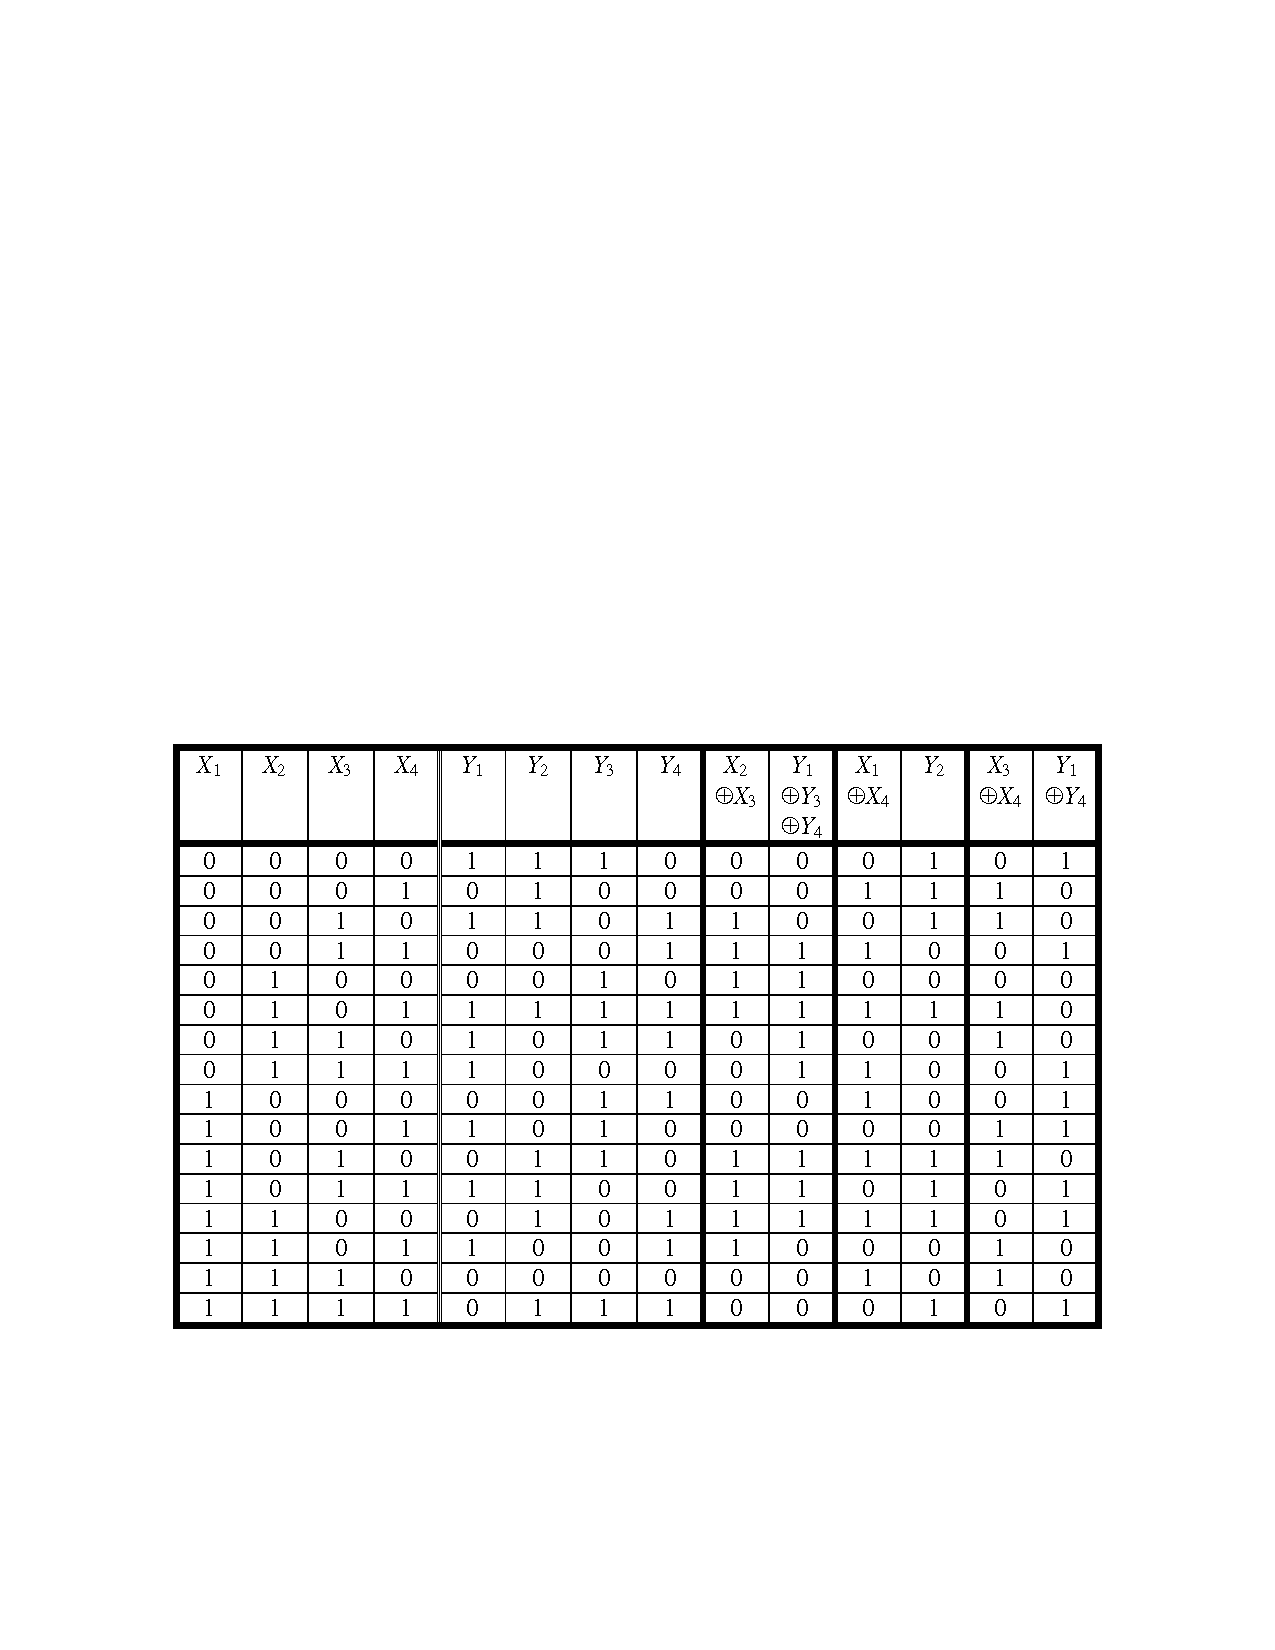
\includegraphics[width=100mm]{pic/linear-sbox} 
\end{center}
\end{figure}
\end{frame}
\begin{frame}\frametitle{An Example of Linear Distribution Table}
\begin{figure}
\begin{center}
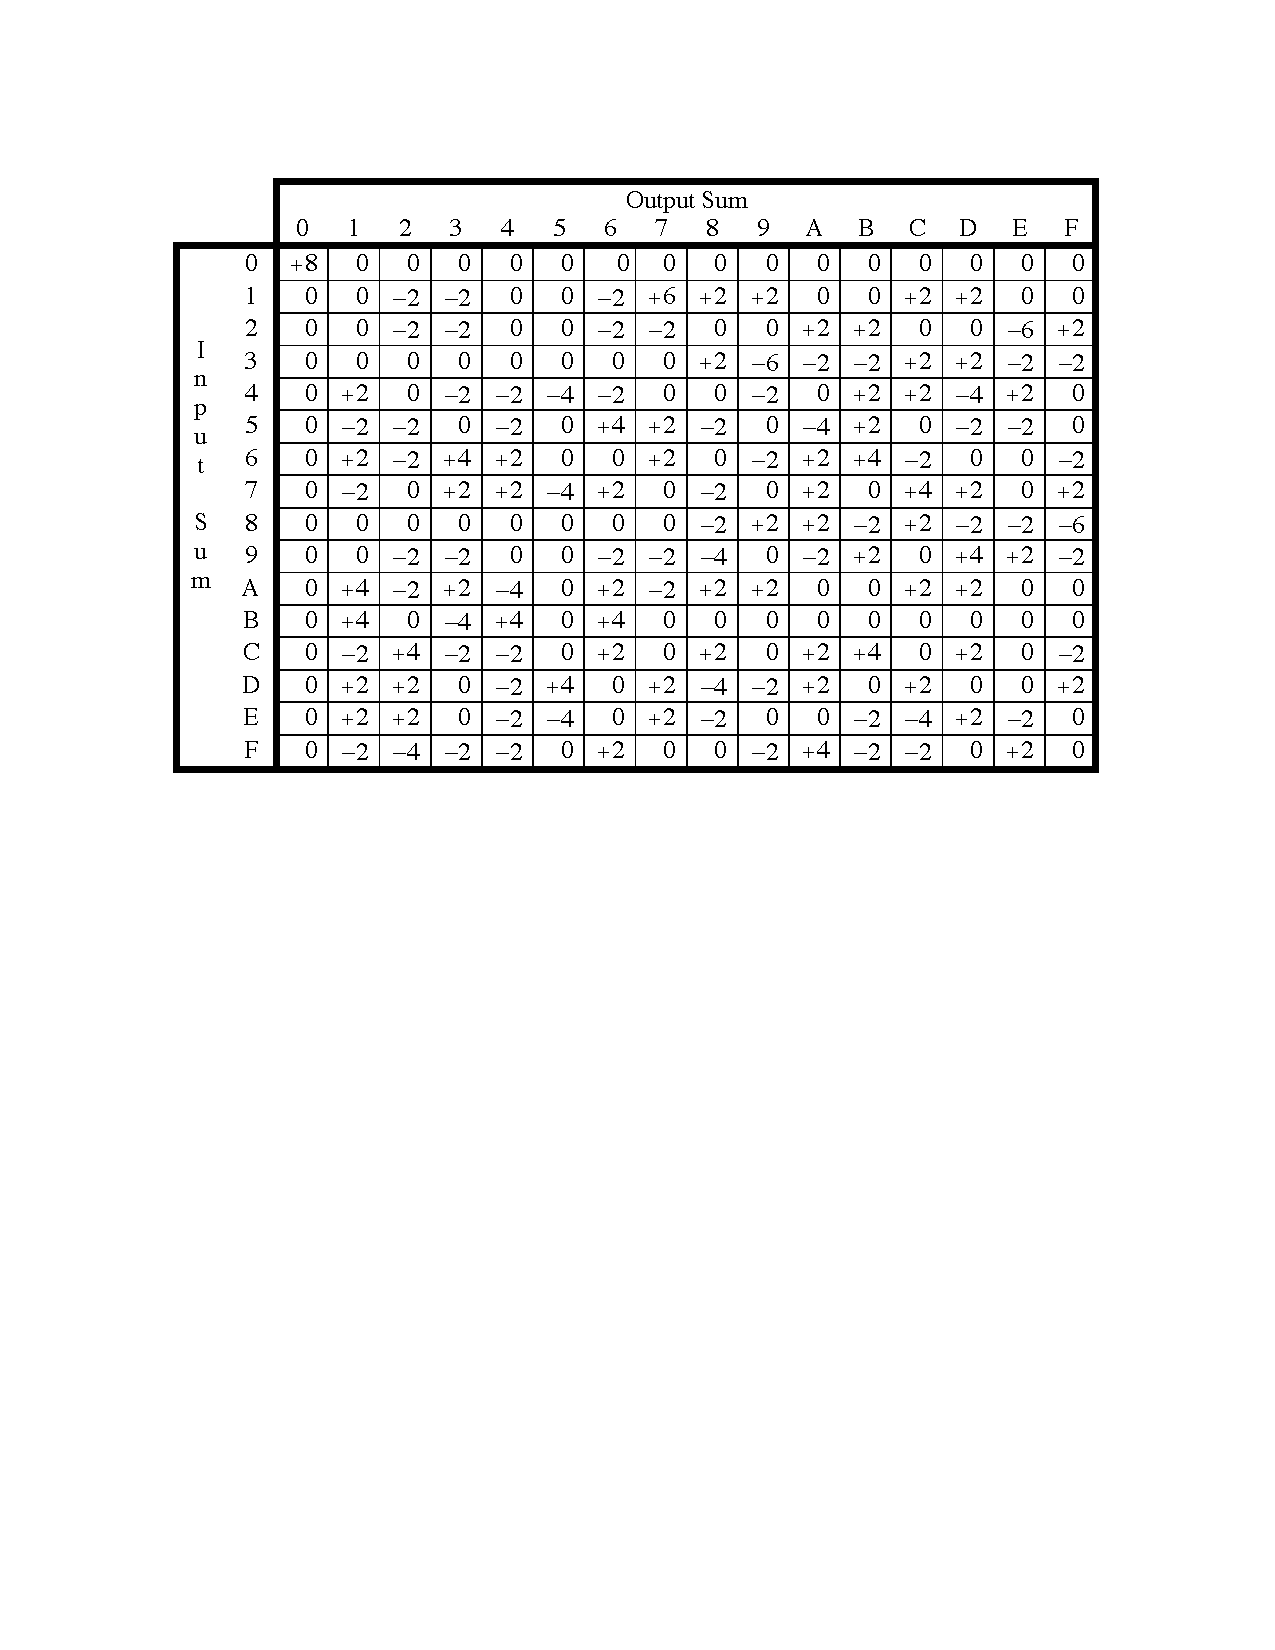
\includegraphics[width=100mm]{pic/linear-table} 
\end{center}
\end{figure}
$x_{2}\oplus x_{3} = y_{1}\oplus y_{3} \oplus y_{4}$ for 12 times, the bias is $12 - 8 =4$ times
$x_{2}\oplus x_{3}: 0110 = 6,\quad y_{1}\oplus y_{3} \oplus y_{4}: 1011=B$, so $(6, B) =4$
\end{frame}
\begin{frame}\frametitle{An Example of Linear Cryptanalysis}
\begin{figure}
\begin{center}
\begin{tikzpicture}[font=\tiny,thin,
	fw/.style={inner sep=0pt, black,fill=white},
	rv/.style={red, very thick}]
\foreach \z in {1, 2,...,3} {
\node (km\z) at ($\z*(0,-2.2cm)$) [minimum width=6cm,rounded corners=1ex,draw] {$K_\z$};
\foreach \x in {1, 2,...,4} {
\node (s\z\x) at ($(km\z)+\x*(1.5cm,0)-(3.75cm,0.7cm)$) [minimum width=1.2cm,rounded corners=1ex,draw] {$S_{\z,\x}$};
}
\foreach \x in {1, 2,...,4} {
\foreach \y in {1, 2,...,4} {
\draw[-] ($(s\z\x.north)+\y*(0.3cm,0)-(0.75cm,0)$) -- +(0,0.22cm);
\draw[-] ($(s\z\x.south)+\y*(0.3cm,0)-(0.75cm,0)$) -- +(0,-0.22cm) -- ($(s\z\y.south)+\x*(0.3cm,0)-(0.75cm,0.8cm)$) -- +(0,-0.22cm);
}
}
}
\foreach \z in {4} {
\node (km\z) at ($\z*(0,-2.2cm)$) [minimum width=6cm,rounded corners=1ex,draw] {$K_\z$};
}
\foreach \x in {1, 2,...,4} {
\foreach \y in {1, 2,...,4} {
\draw[-] ($(s3\x.north)+\y*(0.3cm,0)-(0.75cm,2.2cm)$) -- +(0,0.22cm);
\draw[-] ($(s3\x.south)+\y*(0.3cm,0)-(0.75cm,-5.8cm)$) -- +(0,-0.22cm);
}
}
%\node at ($(s11.north)+1*(0.3cm,0)-(0.75cm,-5.4cm)$) {$P_1$};
%\node at ($(s14.north)+4*(0.3cm,0)-(0.75cm,-5.4cm)$) {$P_{16}$};
%\node at ($(s12.north)+(1.5cm,0)-(0.75cm,-5.4cm)$) {\textbf{Plaintext}};

\node (p5) at ($(s12.north)+1*(0.3cm,0)-(0.75cm,-0.8cm)$) [anchor=south, fw] {\small $p_5$};
\node (p7) at ($(s12.north)+3*(0.3cm,0)-(0.75cm,-0.8cm)$) [anchor=south, fw] {\small $p_7$};
\node (p8) at ($(s12.north)+4*(0.3cm,0)-(0.75cm,-0.8cm)$) [anchor=south, fw] {\small $p_8$};

\draw[rv,-] (p5) -- +(0,-1cm) node [pos=0.42, left,fw] {\small $k_{1,5}$} -- ($(s12.south)+2*(0.3cm,0)-(0.75cm,0)$);
\draw[rv,-] (p7) -- +(0,-1cm) node [pos=0.42, left,fw] {\small $k_{1,7}$} -- ($(s12.south)+2*(0.3cm,0)-(0.75cm,0)$);
\draw[rv,-] (p8) -- +(0,-1cm) node [pos=0.42, right,fw] {\small $k_{1,8}$} -- ($(s12.south)+2*(0.3cm,0)-(0.75cm,0)$);
\draw[rv,-latex] ($(s12.south)+2*(0.3cm,0)-(0.75cm,0)$) -- ($(s32.north)+2*(0.3cm,0)-(0.75cm,0)$) node [pos=0.32, left,fw] {\small $k_{2,6}$} node [pos=0.88, left,fw] {\small $k_{3,6}$} node [pos=1,left, fw] {\small $u_{3,6}$};
\draw[rv,-latex] ($(s22.north)+2*(0.3cm,0)-(0.75cm,0)$) -- ($(s22.south)+4*(0.3cm,0)-(0.75cm,0)$) -- +(0,-0.22cm) -- ($(s24.south)+2*(0.3cm,0)-(0.75cm,0.8cm)$) -- ($(s34.north)+2*(0.3cm,0)-(0.75cm,0)$) node [pos=0.5, left,fw] {\small $k_{3,14}$} node [pos=1,right, fw] {\small $u_{3,14}$};
\node (k41) at (1.5cm,-8.8cm) [fw] {\small $k_{4,2\cdot i}$};
\node (e1) at ($(km1)+5.6*(1.5cm,0)-(3.75cm,0.7cm)$) [fw] {\small $S_{1,2}$: $x_1 \oplus x_3 \oplus x_4 = y_2$};
\node (e2) at ($(km2)+5.4*(1.5cm,0)-(3.75cm,0.7cm)$) [fw] {\small $S_{2,2}$: $x_2 = y_2 \oplus y_4$};
\node (e3) at ($(km3)+5.5*(1.5cm,0)-(3.75cm,0.7cm)$) [fw] {\small $u_{3,6} \oplus u_{3,14} \oplus$};
\node (e4) at ($(km3)+5.5*(1.5cm,0)-(3.75cm,1.2cm)$) [fw] {\small $p_{5} \oplus p_{7} \oplus p_{8} = 0$};
\node (e5) [below of=e4,fw] {\small Guess $k_{4,2\cdot i}$};
\end{tikzpicture}
\end{center}
\end{figure}
\end{frame}
\begin{frame}\frametitle{Differential Cryptanalysis}
\begin{itemize}
\item Specific differences $\Delta_x$ in the input that lead to specific differences $\Delta_y$ in the output with probability $p \gg 2^{-n}$.
\item $x_1\oplus x_2=\Delta_x$, $F_k(x_1) \oplus F_k(x_2)=\Delta_y$ with probability $p$.
\item This can be exploited by CPA.
\item Attack steps:
\begin{enumerate}
\item Construct the difference distribution table of $S$-boxes.
\item Construct a differential characteristics of the first $r-1$ rounds with a big bias.
\item Extracting sub-key bits of last round that satisfies the differential characteristics well.
\end{enumerate}
\end{itemize}
\end{frame}
\begin{frame}\frametitle{An Example of Differential Analysis of $S$-box}
\begin{figure}
\begin{center}
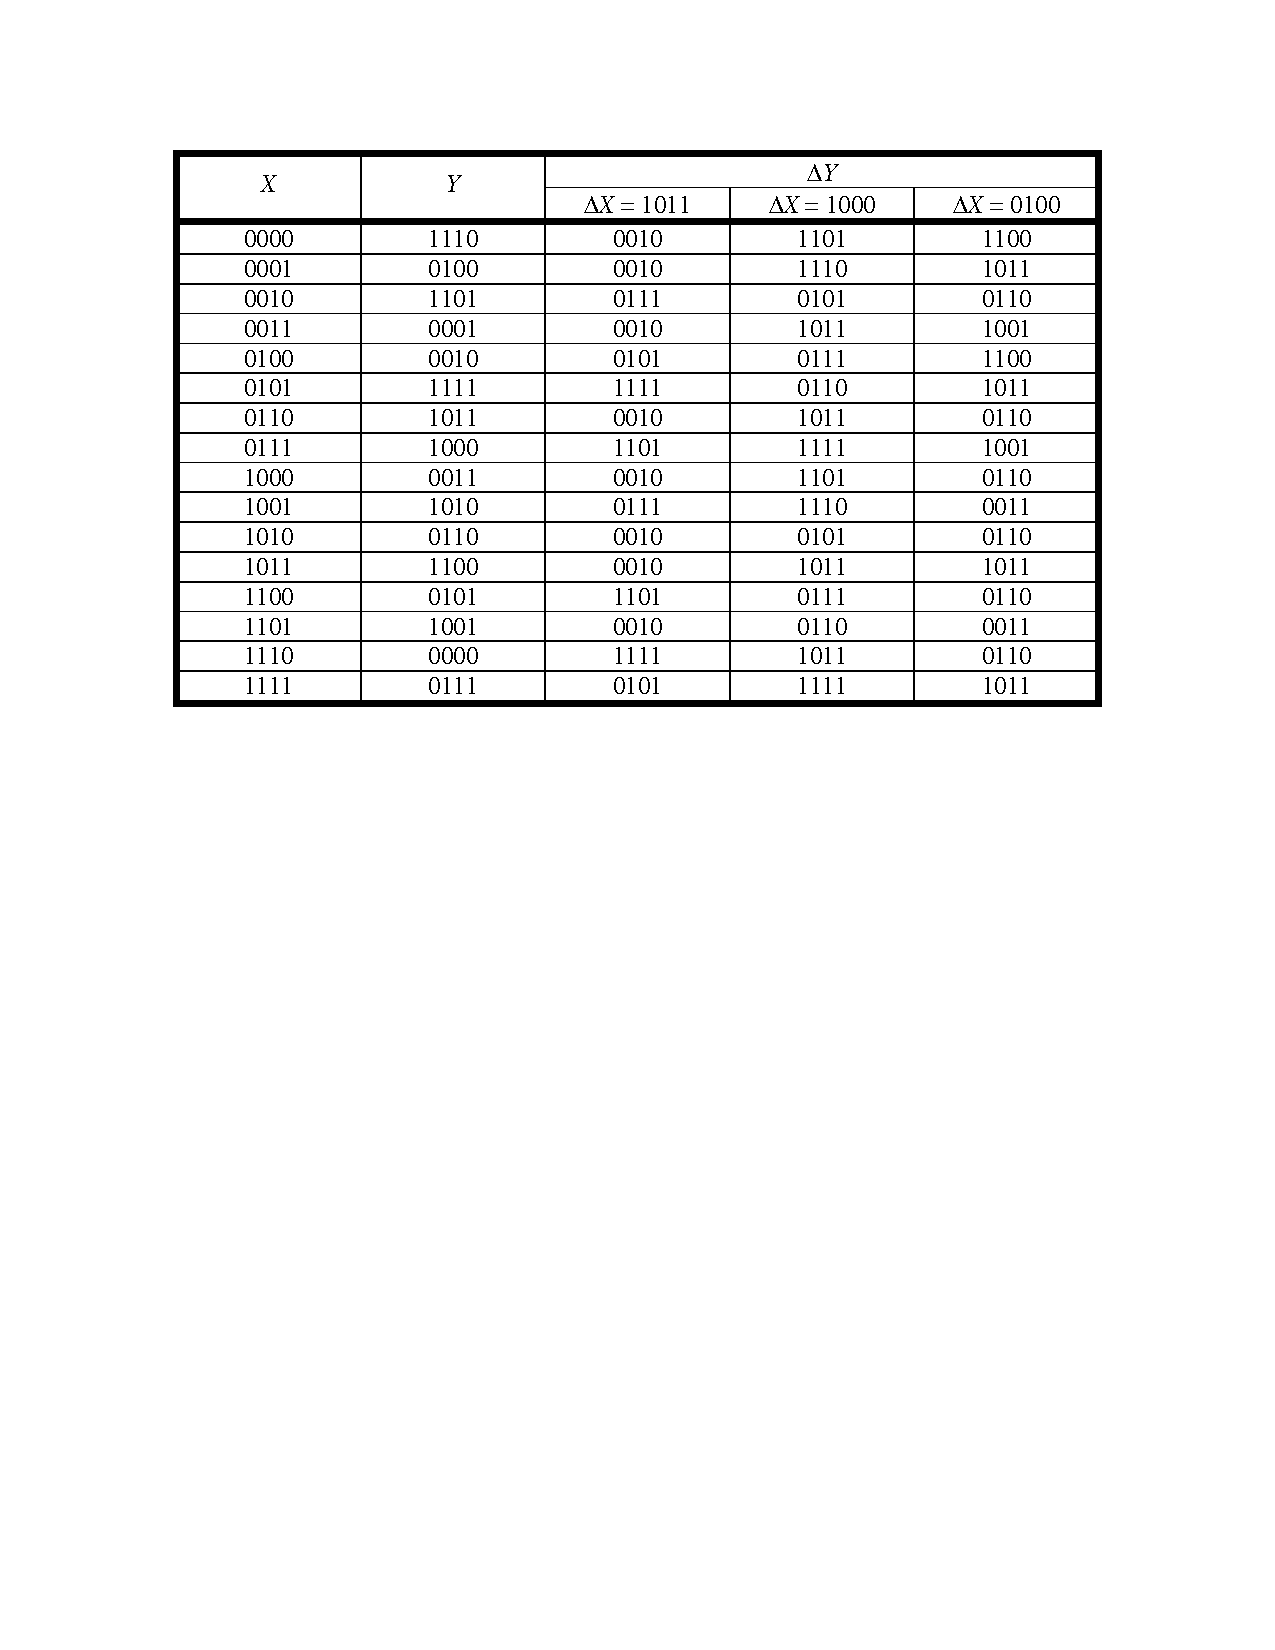
\includegraphics[width=100mm]{pic/difference-sbox} 
\end{center}
\end{figure}
\end{frame}
\begin{frame}\frametitle{An Example of Differential Distribution Table}
\begin{figure}
\begin{center}
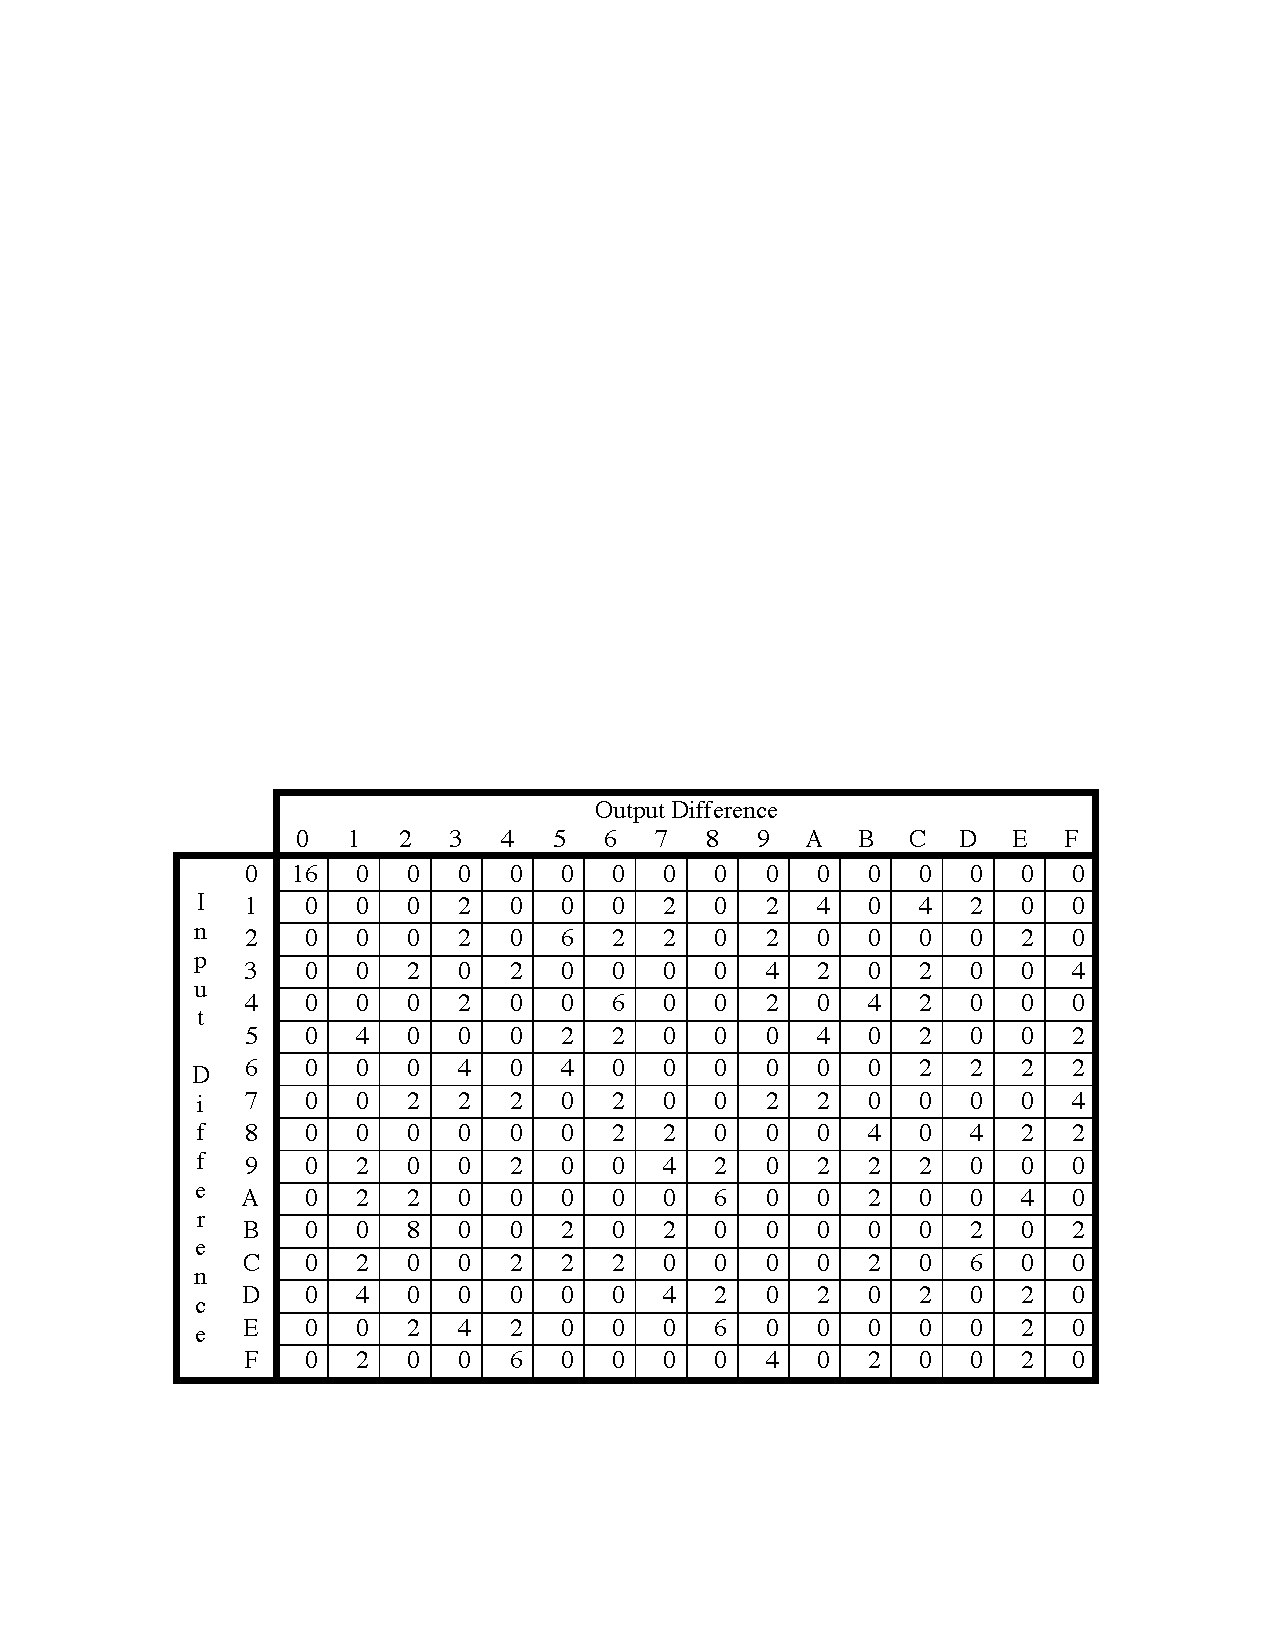
\includegraphics[width=100mm]{pic/difference-table} 
\end{center}
\end{figure}
$\Delta X = 1011 = B, \Delta Y = 0010 = 2$ for 8 times, so $(B, 2) = 8$
\end{frame}
\begin{frame}\frametitle{An Example of Differential Cryptanalysis}
\begin{figure}
\begin{center}
\begin{tikzpicture}[font=\tiny,thin,
	fw/.style={inner sep=0pt, black,fill=white},
	rv/.style={red, very thick}]
\foreach \z in {1, 2,...,3} {
\node (km\z) at ($\z*(0,-2.2cm)$) [minimum width=6cm,rounded corners=1ex,draw] {$K_\z$};
\foreach \x in {1, 2,...,4} {
\node (s\z\x) at ($(km\z)+\x*(1.5cm,0)-(3.75cm,0.7cm)$) [minimum width=1.2cm,rounded corners=1ex,draw] {$S_{\z,\x}$};
}
\foreach \x in {1, 2,...,4} {
\foreach \y in {1, 2,...,4} {
\draw[-] ($(s\z\x.north)+\y*(0.3cm,0)-(0.75cm,0)$) -- +(0,0.22cm);
\draw[-] ($(s\z\x.south)+\y*(0.3cm,0)-(0.75cm,0)$) -- +(0,-0.22cm) -- ($(s\z\y.south)+\x*(0.3cm,0)-(0.75cm,0.8cm)$) -- +(0,-0.22cm);
}
}
}
\foreach \z in {4} {
\node (km\z) at ($\z*(0,-2.2cm)$) [minimum width=6cm,rounded corners=1ex,draw] {$K_\z$};
}
\foreach \x in {1, 2,...,4} {
\foreach \y in {1, 2,...,4} {
\draw[-] ($(s3\x.north)+\y*(0.3cm,0)-(0.75cm,2.2cm)$) -- +(0,0.22cm);
\draw[-] ($(s3\x.south)+\y*(0.3cm,0)-(0.75cm,-5.8cm)$) -- +(0,-0.22cm);
}
}
%\node at ($(s11.north)+1*(0.3cm,0)-(0.75cm,-5.4cm)$) {$P_1$};
%\node at ($(s14.north)+4*(0.3cm,0)-(0.75cm,-5.4cm)$) {$P_{16}$};
%\node at ($(s12.north)+(1.5cm,0)-(0.75cm,-5.4cm)$) {\textbf{Plaintext}};

\node (p5) at ($(s12.north)+1*(0.3cm,0)-(0.75cm,-0.8cm)$) [anchor=south, fw] {};
\node (p7) at ($(s12.north)+3*(0.3cm,0)-(0.75cm,-0.8cm)$) [anchor=south, fw] {\small $\Delta P=$ [0000 1011 0000 0000]};
\node (p8) at ($(s12.north)+4*(0.3cm,0)-(0.75cm,-0.8cm)$) [anchor=south, fw] {};

\draw[rv,-] (p5) -- +(0,-1cm) -- ($(s12.south)+2*(0.3cm,0)-(0.75cm,0)$);
\draw[rv,-] (p7) -- +(0,-1cm) -- ($(s12.south)+2*(0.3cm,0)-(0.75cm,0)$);
\draw[rv,-] (p8) -- +(0,-1cm) -- ($(s12.south)+2*(0.3cm,0)-(0.75cm,0)$);
\draw[rv,-latex] ($(s12.south)+2*(0.3cm,0)-(0.75cm,0)$) -- ($(s32.north)+2*(0.3cm,0)-(0.75cm,0)$)  node [pos=1,left, fw] {\small $u_{3,6}$};
\draw[rv,-latex] ($(s22.north)+2*(0.3cm,0)-(0.75cm,0)$) -- ($(s22.south)+4*(0.3cm,0)-(0.75cm,0)$) -- +(0,-0.22cm) -- ($(s24.south)+2*(0.3cm,0)-(0.75cm,0.8cm)$) -- ($(s34.north)+2*(0.3cm,0)-(0.75cm,0)$) node [pos=1,right, fw] {\small $u_{3,14}$};
\node (k41) at (1.5cm,-8.8cm) [fw] {\small $k_{4,2\cdot i}$};
\node (e1) at ($(km1)+5.8*(1.5cm,0)-(3.75cm,0.7cm)$) [fw] {\small $S_{1,2}$: $\Delta X = B \to \Delta Y = 4$};
\node (e2) at ($(km2)+5.8*(1.5cm,0)-(3.75cm,0.7cm)$) [fw] {\small $S_{2,2}$: $\Delta X = 4 \to \Delta Y = 5$};
\node (e3) at ($(km3)+5.9*(1.5cm,0)-(3.75cm,0.7cm)$) [fw] {\small $\Delta U=$ [0000 0100 0000 0100]};
\node (e4) at ($(km3)+5.5*(1.5cm,0)-(3.75cm,1.2cm)$) [fw] {};
\node (e5) [below of=e4,fw] {\small Guess $k_{4,2\cdot i}$};
\end{tikzpicture}
\end{center}
\end{figure}
\end{frame}
%\end{comment}
\begin{frame}\frametitle{Remarks on Block Ciphers}
\begin{itemize}
\item \textbf{Block length} should be sufficiently large
\item \textbf{Message tampering} is not with message confidentiality
\item \textbf{Padding}: TLS: For $n>0$, $n$ byte pad is $n,n,\dots,n$
If no pad needed, add a dummy block
\item \textbf{Stream ciphers vs. block ciphers}: 
\begin{itemize}
\item Steam ciphers are faster but have lower security
\item It is possible to use block ciphers in ``stream-cipher mode''
\end{itemize}
\end{itemize}
\begin{exampleblock}{Performance: Crypto++ 5.6, AMD Opetron 2.2GHz}
\begin{center}
\begin{tabular}{|c|c|c|} \hline
                      & \textbf{Block/key size} & \textbf{Speed MB/sec} \\ \hline
\textbf{RC4}          &         & 126 \\  
\textbf{Salsa20/12}   &         & 643 \\ 
\textbf{Sosemanuk}    &         & 727 \\ 
\textbf{3DES}	      & 64/168  & 13  \\
\textbf{AES-128}      & 128/128 & 109 \\ \hline 
\end{tabular}	
\end{center}
\end{exampleblock}
\end{frame}
\begin{frame}\frametitle{Comics on S-box [xkcd:153]}
If you got a big keyspace, let me search it.
\begin{figure}
\begin{center}
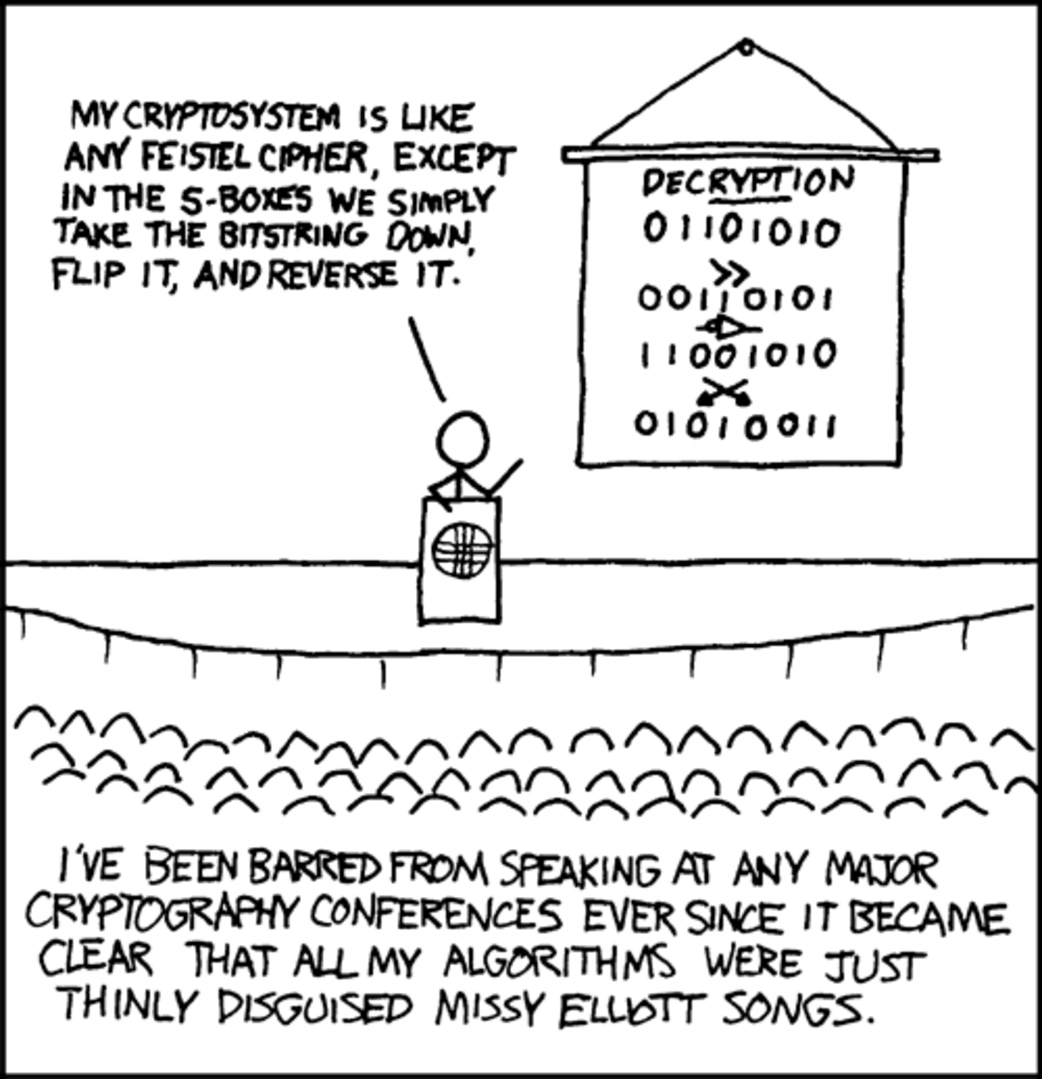
\includegraphics[width=70mm]{pic/sbox-talk} 
\end{center}
\end{figure}
\end{frame}
\begin{frame}\frametitle{Summary}
\begin{itemize}
\item Block cipher is PRP.
\item confusion \& diffusion, SPN, Feistel network, avalanche effect.
\item DES, 3DES, AES.
\item reduced round, meet-in-the-middle, differential and linear cryptanalysis. 
\end{itemize}
\end{frame}
\end{document}